\chapter{METHODOLOGY AND RESULTS}
\label{ch:methodology-results}

% Overview of chapter
\section{Overview}

% About the hypotheses and objectives
% About the user selection criteria
In this chapter, we briefly revisit the objectives of this work to formulate the hypotheses and methodology for our experiment. We establish the selection criteria for the users in our experiment, which enforce restrictions to provide a more controllable environment given societarial restrictions inherent to the time at which this work was developed.

% About the classification of the user base
% About the methodology of the experiment
We specify the classification method used in this experiment, which was employed to compare the effects of our DDA system to different types of users, in comparison to the traditional fixed difficulty presets commonly seen in commercial games. In sequence, we explain the methodology used in our experiment, specifying the division of user groups, describing the metrics used to compare such groups, providing a brief description of the steps performed by users in the experiment, and providing details on a survey used to assess user perceptions after performing the experiment.

% About the analysis of results 
Finally, we report and analyze the results of our experiment, performing a comparison of the performance of user groups when using DDA systems or fixed difficulty. We perform a more granular comparison by separating  the data for each group based on our initial user classification, and assess the effects of DDA systems on each player profile: \emph{beginners}, \emph{intermediates} and \emph{veterans}. We also compare the performance of players to their own assessment of the difficulty of our game, and correlate their perception with our performance analysis.

% ======================================================================
% ======================================================================
% =================================================================

\section{Hypotheses and Objectives}
\label{sec:hypotheses-and-objectives}

% Main Objectives
% ===================
%       - Verify if dynamic adjustments create an increase in the performance over the play session for beginner & intermediate players
%       - Verify if dynamic adjustments keep a fair challenge, without overt increases in performance for advanced players
As a first objective when performing this experiment, we wish to verify if dynamic adjustments can create a relevant increase in player performance in the first or second playthrough for players that are inexperienced with \emph{Souls-like} games. We attempt to understand if players that experience dynamic difficulty at their first playthrough can achieve a better understanding of game mechanics on their second playthrough.

We also wish to understand if dynamic difficulty can maintain a fair level of challenge to veterans or experienced players on a second playthrough. To do this, we wish to evaluate the difference in performance between fixed and dynamic difficulty on a second playthrough where players have likely increased their performance when using game mechanics. Based on these objectives, we formulate the following hypotheses:

% * Hypotheses
% * ====================================
% Hypothesis 1: Dynamic can alleviate the learning curve for beginners
% Hypothesis 2: Dynamic is less frustrating than fixed for beginners
% Hypothesis 3: Dynamic can keep a better challenge on 2nd+ playthrough
% Hypothesis 4: Dynamic is not overtly easy to veterans
\begin{itemize}
    \item{Hypothesis 1: Dynamic difficulty can alleviate the steep learning curve of challenging games for inexperienced players;}
    \item{Hypothesis 2: Dynamic difficulty can provide a better suited level of challenge on the second or subsequent playthroughs.}
\end{itemize}

The hypotheses defined have the intent of comparing DDA systems to fixed difficulty on two different aspects: the ability for players to learn and become used to \emph{Souls-like} game mechanics in a first playthrough, and the ability for the game to provide a sufficient level of challenge to players which have become accustomed to and proficient at the game at a second or subsequent playthrough.

% Validation of Hypothesis 1
% =========================

% Most common causes of failure are discovery
As discussed in chapter \label{ch:analysis-dark-souls}, the most prevalent causes of failure in a first playthrough in \emph{Souls-like} games are becoming used to the game's input and its resulting actions, understanding the principles of the most relevant game mechanics, and memorizing patterns of enemies or level layouts. In a second playthrough, players will generally have achieved a consolidated understanding of which elements provide the most significant challenge, and how to use the game's mechanics in a way that maximizes their chances of success.

% We wish to validate that 
Therefore, failure is often part of the process of learning in a first playthrough. Presenting the player with a slight difficulty spike at a specific point in the game could be a tool to accelerate the process of learning a specific game mechanic, given that the level of challenge is not overtly contrasted to the player's skill. Thus, we wish to validate our hypothesis that the performance of players which experience Dynamic Difficulty first is higher than those which experience fixed difficulty first, as they become used to the game's mechanics and challenges.

% Validation of hypothesis 1
To perform the validation of Hypothesis 1, we divide the users in our experiment in two groups: users which experience Fixed Difficulty first (Group A), and users which experience Dynamic Difficulty systems first (Group B). After performing such division, we must evaluate the performance of each group according to level progression in their first playthrough, by gathering multiple performance statistics for each level. To validate the hypothesis, we must validate that the average performance of Group B is higher than the performance of Group A. Therefore, the \emph{null hypothesis} of Hypothesis 1 is that the average performance of Group A is the same or higher than the performance of Group B.

% Validation of Hypothesis 2
% =========================

In a second playthrough, players will have experienced and become used to most or all relevant game mechanics or difficulty factors. In consequence, most players will be able to devise one or multiple plans of action against challenging elements ahead of time, and attempt to execute such plans. 

Therefore, the most prevalent cause of failure in a second playthrough with fixed difficulty is a failure of execution, where the player either performs their input incorrectly, or their plan of action does not optimally address the issues inherent to a specific challenge. As a consequence, players will generally present a much better performance in a second playthrough in fixed difficulty systems.

However, when the advent of dynamic difficulty is employed, the game is able to present new challenges and situations, and even increase the complexity at which a game mechanic needs to be executed by the player. Therefore, even though players are used to most or all game mechanics in a second playthrough, their performance can stay at the same or a lower level than that of the first playthrough. Therefore, we wish to evaluate the performance of players in a second playthrough, which occurs in the second part of the experiment.

To validate Hypothesis 2, we wish to verify that the average performance of Group A (which starts with fixed difficulty) is the same or lower than the average performance of Group B (which starts with dynamic difficulty). Therefore, the \emph{null hypothesis} of Hypothesis 2 is that the average performance of Group B is significantly higher than that of Group A in a second playthrough.

% =================================================================

% * Scenarios
% * ====================================

% * Variables
% * ====================================

% =================================================================
% =================================================================
% =================================================================

\section{User Selection Criteria}
\label{sec:user-selection-criteria}
% * User selection criteria
% * ====================================

\sepfootnotecontent{fn:bloodborne}{Bloodborne (FromSoftware, 2015). Video Game. Available on PlayStation 4.}
\sepfootnotecontent{fn:sekiro}{Sekiro: Shadows Die Twice (FromSoftware, 2019). Video Game. Available on PlayStation 4, Xbox One, Microsoft Windows, Google Stadia.}
\sepfootnotecontent{fn:steam}{\emph{Steam} is an online storefront and a digital service for video game distribution, developed by \emph{Valve}. Features provided by Steam include digital rights management, social networking, cloud-based game saving systems, automatic game updating and streaming.}

The methodology used for our experiment involves the deployment and use of our application in environments where the users are comfortable playing, without in-person monitoring by the experiment observers. For the analysis of user performance and results, we remotely collect data through telemetry, and compare data sets based on user classification and use the results of our player perception surveys as a reference. We employed restricted selection criteria for our user base to ensure similar characteristics on how the application is used.

The selection of users for our experiment was guided by a small set of profile characteristics and hardware requirements. This was required to mitigate the impact of external and unmanageable factors such as preferences, age, platform or input devices to the performance of users. Users were invited for the experiment through multiple Brazilian online gaming communities using the \emph{Discord} application. The targeted groups included communities with players of all skill levels, with the shared common interest of discussing  \emph{Souls-like} games, such as \emph{Dark Souls}, \emph{Bloodborne}\sepfootnote{fn:bloodborne} and \emph{Sekiro}\sepfootnote{fn:sekiro}. We define in the list below the profile-based criteria for user selection performed in our experiment:
% Player profile
% ===================
%   - Age: 18-23
%   - Plays Console or PC video games
%   - Prefers the use of joystick controllers
%   - Has a Steam account
\begin{itemize}
    \item{\emph{Age:} between 18 and 23 years old;}
    \item{\emph{Preffered gaming platforms:} Video Game Consoles or Desktop PC;}
    \item{\emph{Preffered input methods:} dual-analog joysticks;}
    \item{\emph{Additional requirements:} has a Steam\sepfootnote{fn:steam} account.}
\end{itemize}

% \subsection{Hardware Requirements}
% Hardware requirements
% ===================
We also require users to possess hardware that satisfies the proper execution of our application under a target framerate of 60 frames per second, to ensure that player performance is not affected by low graphical performance, stuttering or input lag. In the list below we specify the hardware requirements to properly execute our application under our specified hardware performance targets:
% Hardware Requirements \\
% 64 bit processor and Operating System \\
% Processor: Intel Core i5-2300 2.8GHz+ or AMD FX-6300 3.5GHz+ \\
% Graphics: NVIDIA GeForce GTX 460 or AMD Radeon 5000 series+ \\
% DirectX: Version 11+ \\
% Operating System: Windows 7 64bit, Service Pack 1+ \\
% Memory: 6GB+ RAM \\
% Available Storage: 4GB+ available on HDD or SSD \\
% 16:9 or 16:10 monitor between 19" and 24" and at least 1280x720 native resolution \\
\begin{itemize}
    \item{\emph{System Architecture:} 64 bit processor and Operating System;}
    \item{\emph{Processor:} Intel Core i5-2300 2.8GHz+ or AMD FX-6300 3.5GHz+;}
    \item{\emph{Graphics:} NVIDIA GeForce GTX 460 or AMD Radeon 5000 series+;}
    \item{\emph{DirectX:} Version 11+;}
    \item{\emph{Operating System:} Windows 7 64bit, Service Pack 1+}
    \item{\emph{Memory:} 6GB+ RAM}
    \item{\emph{Available Storage:} 4GB+ available on HDD or SSD}
    \item{\emph{Display:} 16:9 or 16:10 monitor sized between 19" and 32" and at least 1280x720 native resolution.}
\end{itemize}

% \subsection{Required Peripherals \& Input Methods}
We also require that players use similar input interface methods, to ensure that the accuracy of performed actions such as character movement, camera movement, dodging or blocking are not affected by restrictions on input devices, such as a computer keyboard not being able to represent directional movement with the same level of freedom as a dual-analog joystick. In the following list we specify the characteristics used to define the input interfaces required to be used by players in our experiment:  
% Required Peripherals & Input
% ===================
% Required peripherals and input: \\
%  - Joystick controller:  \\
%      - Xbox Controllers: Xbox 360, Xbox One, Xbox Series X \\
%      - Playstation Controllers: DualShock 3, Dual Shock 4, Dual Sense \\
%      - Or equivalent models with at least: \\
%          - Dual analogs \\
%          - 4 face buttons \\
%          - 4 digital directional buttons \\
%          - Right and left triggers and bumpers
\begin{itemize}
    \item{\emph{Xbox Controllers:} Xbox 360, Xbox One, Xbox Series X;}
    \item{\emph{PlayStation Controllers:} DualShock 3, DualShock 4, Dual Sense;}
    \item{\emph{Equivalent Joystick Controller Models} with at least:}
    \begin{itemize}
        \item{Dual Analog axes, one at each side;}
        \item{A clickable Trigger Button at each analog axis;}
        \item{4 Face Buttons in the right side;}
        \item{4 Digital Directional Buttons in the left side;}
        \item{Right and Left Triggers and Bumpers at the top.}
    \end{itemize}
\end{itemize}

We apply some of the aforementioned criteria through a \emph{Player Classification Survey}, which is further detailed in section \ref{sec:user-base-classification}. The Player Classification survey is also used to categorize our users in skill-based classification groups, such as \emph{Beginner}, \emph{Intermediate} and \emph{Veteran} users. Information on the specific questions and metrics used in the classification survey can be seen in appendix \ref{anx:player-classification-survey}. Regarding the topics not covered in the classification survey, we applied a secondary \emph{Player Experiment Requirements Survey}, which can be seen in \ref{anx:player-experiment-requirements-survey}

% TODO add photo of how the environment for the experiment was supposed to be

% =================================================================
% =================================================================
% =================================================================

\section{Classification of the User Base}
\label{sec:user-base-classification}
% * User classification groups
% * ====================================

We define user classification groups which are used to divide our data sets based on expected levels of player skill. Such classification is necessary to evaluate the impact of difficulty and dynamic difficulty adjustments based on player expertise. Additionally, we also use such classification to evaluate the opinions of different players on the validity of our application as a sufficient representative of the core aspects of our object of study, \emph{Dark Souls}. The classification is performed based on a \emph{Player Classification Survey}, which was performed during the User Selection step of our experiment.

% Objective
% ===================
%   - Separate players in beginners, intermediate, veterans
%       - Beginners: casuals, unused to action games
%       - Intermediate: average, used to action games
%       - Veterans:  hardcore, used to action & Souls-like games

% Classification Groups
% ===================
%   - Beginners:
%       - Never played a souls-like
%       - Low experience in action games
%       - Low avg. playtime
%   - Intermediate
%       - Previously played souls-likes
%       - Never finished a souls-like
%       - Medium or high experience in action games
%       - Moderate or high avg. playtime
%   - Veterans
%       - Finished one or multiple souls-likes
%       - High experience in action games
%       - High avg. playtime

We separate the player base in our experiment in the following groups: \emph{beginners}, \emph{intermediate} and \emph{veterans}. We define general descriptions for each group to serve as a guide when defining functional and data-based metrics which can be applied to our Player Classification Survey:

\begin{itemize}
    \item{\emph{Beginners:} casual players which are unused to playing action games, or players which are initiating their first playthrough on a \emph{Souls-like} game;}
    \item{\emph{Intermediate:} recurrent players which are used to action games, and have finished or relevantly progressed through a single \emph{Souls-like} game;}
    \item{\emph{Veterans:} dedicated players which are used to the \emph{Souls-like} genre, and have finished multiple games of FromSoftware's \emph{Souls} franchise.}
\end{itemize}

% Metrics
% ===================
%   - Avg. Playtime per Week
%   - Experience in action games
%   - Completion of Souls-likes

With such descriptions, we can begin to specify each categorization in functional or data-based terminology. We use the definitions of \emph{casual} and \emph{hardcore} players from the work of  \citet{ARTICLE_CasualsHardcoreDefinition} as a reference, where casual players are defined as individuals which perform the act of play \emph{casually} -- who dedicate a smaller portion of their time to play games, and usually on a more restricted set of genres.

Therefore, we define \emph{beginner} players as players with a weekly playtime between 0 and 3 hours, which are comfortable with at most three different game genres which do not include action games, and have not achieved 50\% completion on a \emph{Souls-like} game. \emph{Intermediate} players have a weekly playtime between 4 and 10 hours, are comfortable with at least three game genres which include action games, and have achieved at least 50\% completion on a single \emph{Souls-like} game. \emph{Veteran} players have a weekly playtime above 10 hours, have at least four comfortable game genres which include action games, and have completed two or more \emph{Souls-like} games.

% User base
% ===================
%   - Total number: 23
%       - Beginners: 10
%       - Intermediates: 7
%       - Veterans: 6

The total number of users which participated in ther experiment and sufficiently satisfied our selection criteria was 23, where 10 users were classified as \emph{beginners}, 7 users were classified as \emph{intermediates}, and 6 users were classified as \emph{veterans}. As will be explained in section \ref{sec:experiment-methodology}, we divided our total user base in two groups. Unfortunately, we were unable to acquire an even number of intermediate candidates for a symmetrical division, and the number of intermediate and veteran candidates was significantly lower than than the number of casual players which applied.

Table \ref{tab:user-base-sizes} specifies the definition used in our experiment for each user category, as well as the amount of users in each category which participated in our experiment.

% Event Instance
%   • Timestamp ( Time : double )
%   • Name ( String )
%   • Category ( String )
%   • Source ( ObjectId : GUID )
%   • Params[]
%       • { "name", "type", "value" }

% Table with user classifications
\begin{table}[!ht]
    \begin{center}
      \caption{Users for each user classification category in our experiment.}
      \label{tab:user-base-sizes}
      \rowcolors{2}{}{gray!25} % Alternate row colors
      \begin{tabular}{ w{l}{5em} w{r}{2em} m{25em} } % alignments and column size
        \addlinespace
        \toprule
        % Headings
        \bf Group & \bf Users  & \bf Definition \\
        \midrule
        % Data
        Beginners & 10 & Weekly playtime between 0 and 3 hours; Comfortable with at most 3 different genres different than action games; Have not achieved 50\% completion on a \emph{Souls-like} game. \\
        Intermediate & 7 & Weekly playtime between 4 and 10 hours; Comfortable with at least 3 game genres which include action games; Have achieved at least 50\% completion on a single \emph{Souls-like} game. \\
        Veterans & 6 & Weekly playtime above 10 hours; Have at least 4 comfortable game genres which include action games; Have completed two or more \emph{Souls-like} games. \\
        Total & 23 & All players in our experiment. \\
        \bottomrule
      \end{tabular}
    \end{center}
\end{table}

% =================================================================
% =================================================================
% =================================================================

\section{Experiment Methodology}
% * Experiment 2: Validation of Adaptive Solution
% * ====================================
\label{sec:experiment-methodology}

% * Methodology
% * =======================

\subsection{User Groups}

% Division of user groups
% ===================
%   - Group A: Fixed first, adaptive second
%       - Segment 1: Fixed difficulty modes
%       - Segment 2: N-dimensional adaptive difficulty
%   - Group B: Adaptive first, fixed second
%       - Segment 1: N-dimensional adaptive difficulty
%       - Segment 2: Fixed difficulty modes

As specified in the earlier sections of this chapter, we divide our user base in two similarly sized groups to evaluate the effects of DDA systems in the learning curve for beginners and in the challenge level for proficient players:
\begin{itemize}
    \item{Group A: Fixed Difficulty in the first playthrough (Part 1), and Dynamic Difficulty in the second playthrough (Part 2);}
    \item{Group B: Dynamic Difficulty in the first playthrough (Part 1), and Fixed Difficulty in the second playthrough (Part 2).}
\end{itemize}

% Number in user groups
% ===================
%   - Group A: 12
%       - Beginners: 5
%       - Intermediates: 4
%       - Veterans: 3
%   - Group B: 11
%       - Beginners:  5
%       - Intermediates: 3
%       - Veterans: 3

We attempted to divide our user base simetrically based on each category, as a means to attempt to compare the statistics of each group with the same sample size. Each group contains the same or a similar amount of users for each classification described in section \ref{sec:user-base-classification}. As a result, \emph{Group A} consisted of a total amount of 12 users, with 5 beginners, 4 intermediates and 3 veterans. \emph{Group B} consisted of 11 users, with 5 beginners, 4 intermediates and 3 veterans. Figure \ref{fig:user-group-sizes} illustrates the division and sample size of each user group, separating each group in the classifications defined in section \ref{sec:user-base-classification}.

% Figure with consolidated user group numbers
\begin{figure}[!ht]
    \begin{center}
    \caption{Chart representing the size of each experiment group, separated by our user classification.}
        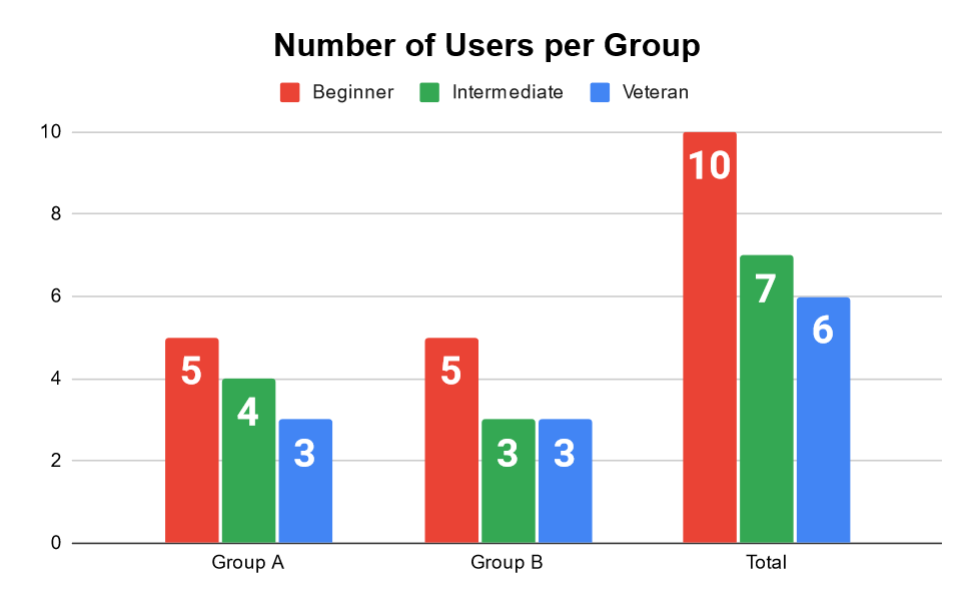
\includegraphics[width=22em]{figures/fig-user-groups.png}
        \legend{Source: Chart assembled by authors.}
        \label{fig:user-group-sizes}
    \end{center}
\end{figure}

\subsection{Experiment Flow}

% Experiment overview
% ===================
%   - Step 1: Perform player classification survey
%       - Be classified as beginner, intermediate, 
%   - Step 2: Be assigned to Group A or Group B
%   - Step 3: Play through part 1
%   - Step 4: Play through part 2
%   - Step 5: Perform player perception & comparison survey

Regarding the execution of our experiment, we defined a series of steps to be performed by users for the authors to be able to classify and divide users, and in sequence collect the performance and perception data of users:

\begin{enumerate}
    \item{User performs the Player Classification Survey;}
    \item{User is classified as a Beginner, Intermediate or Veteran;}
    \item{User is assigned to Group A or Group B;}
    \item{User plays through Part 1 of the Experiment (First Playthrough);}
    \item{User plays through Part 2 of the Experiment (Second Playthrough);}
    \item{User performs the Player Perception Survey.}
\end{enumerate}

% Figure with consolidated user group numbers
\begin{figure}[!ht]
    \begin{center}
    \caption{Diagram representing the steps performed by users in our experiment.}
        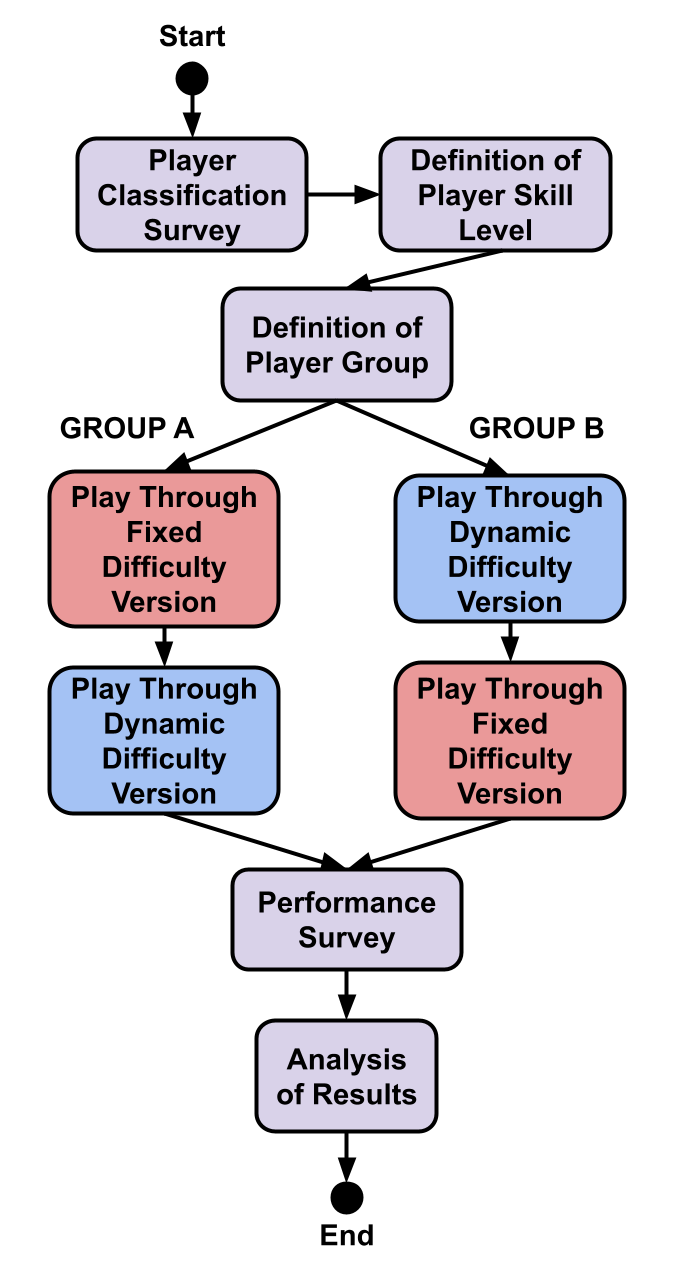
\includegraphics[width=17em]{figures/fig-experiment-flow.png}
        \legend{Source: Diagram assembled by authors.}
        \label{fig:experiment-flow}
    \end{center}
\end{figure}

Figure \ref{fig:experiment-flow} illustrates the aforementioned process in the form of a diagram. There are additional steps which were occluded due to being unrelated to the process of acquiring and evaluating data for the purpose of our experiment. For instance, between a user performing the Player Classification Survey and being classified, users also performed the Experiment Requirement Survey, as it was a necessary step to evaluate if the user hardware was performant enough to run our application.

Additionally, it is important to note that there was no automated method assign users to a classification or a group. Instead, the authors of this work manually analyzed the data and classified users based on observable clusters of data. For the definition of which users would be assigned to each group, a simple symmetrical division was performed without considering any classification-based metrics.

\subsection{Metrics}

% Explanation of used Metrics
% ===================

% Negative Metrics (lower is better)
%   - Avg. Completion Time per Level
%   - Avg. Number of Deaths Per Level
%   - Avg. Health Lost Per Encounter

% Positive Metrics (higher is better)
%   - Avg. Attack Avoidance Efficiency
%   - Avg. Attack Window Efficiency
%   - ? Avg. Damage Dealt Per 10s In Encounters
%   - ? Avg. Stamina Level In Encounters

% Table with Descriptions for Performance Metrics used for Evaluating Player Performance
\begin{table}[!ht]
    \begin{center}
      \caption{Descriptions of the Performance Metrics used to evaluate Players.}
      \label{tab:descriptions-performance-metrics}
      \rowcolors{2}{}{gray!25} % Alternate row colors
      \begin{tabular}{ m{6em} m{27em} } % alignments and column size
        \addlinespace
        \toprule
        % Headings
        \bf Metric & \bf Description  \\
        \midrule
        % Data
        \makecell[c]{Adjustment\\Target} & \\
        \makecell[c]{Attack\\Avoidance\\Efficiency} & \\
        \makecell[c]{Attack\\Window\\Efficiency} & \\
        \makecell[c]{Completion\\Time} & \\
        \makecell[c]{Damage Dealt\\per 10 seconds} & \\
        \makecell[c]{Deaths per\\Level} & \\
        \makecell[c]{Health Lost\\per Encounter} & \\
        \bottomrule
      \end{tabular}
    \end{center}
\end{table}

\subsection{Player Perception Survey}
% Player Perception & Comparison Survey Motivation and Details
% ===================

%   - Verify if gameplay, aesthetics and challenge meet player expectations for a Dark Souls replica
%   - Observe performance metrics & define adjustment thresholds

% TODO add table with the questions and their objective

% TODO Add annex with the Player Perception Survey

% =================================================================
% =================================================================
% =================================================================

\section{Results}
% * Results
% * =======================

\subsection{Perceptions on Usability and Fidelity of All Players}

%   - Player Perception Survey
%       - Perception on Aesthetic Fidelity
%       - Perception on Gameplay Fidelity
%       - Peception on Usability

% =================================================================
% =================================================================
% =================================================================

\subsection{Beginner Players}

% Perception
% =============================

% Performance
% =============================

% Table with Observations for Performance Metrics for Beginner Players
\begin{table}[!ht]
    \begin{center}
      \caption{Observations on Performance Metrics for Beginner Players.}
      \label{tab:observations-performance-metrics-beginners}
      \rowcolors{2}{}{gray!25} % Alternate row colors
      \begin{tabular}{ w{c}{6em} m{27em} } % alignments and column size
        \addlinespace
        \toprule
        % Headings
        \bf Metric & \bf Observations  \\
        \midrule
        % Data
        \makecell[c]{Adjustment\\Target} & \\
        \makecell[c]{Attack\\Avoidance\\Efficiency} & \\
        \makecell[c]{Attack\\Window\\Efficiency} & \\
        \makecell[c]{Completion\\Time} & \\
        \makecell[c]{Damage Dealt\\per 10 seconds} & \\
        \makecell[c]{Deaths per\\Level} & \\
        \makecell[c]{Health Lost\\per Encounter} & \\
        \bottomrule
      \end{tabular}
    \end{center}
\end{table}

%adjustment_target_level
% Avg Adjustment Target per Level - Beginners
% =======================
\begin{figure}[!ht]
    \begin{center}
    \caption{Avg. Adjustment Target (Y) per Level (X) for Beginners.}
        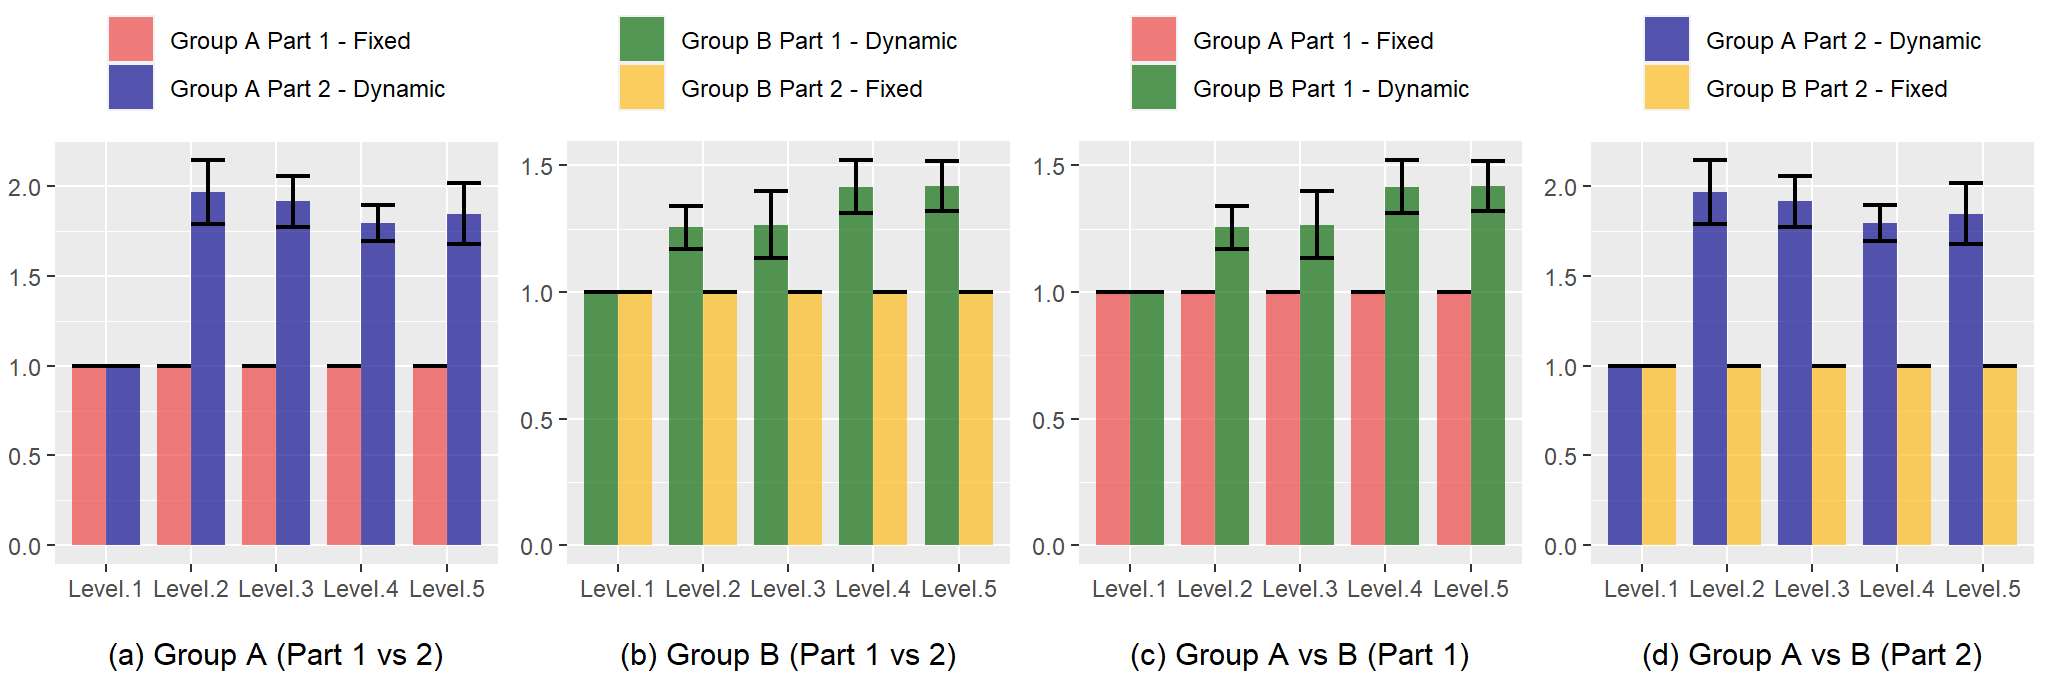
\includegraphics[width=34em]{figures/adjustment_target_level-beginner_players.png}
        \legend{Source: Assembled by authors.}
        \label{fig:result-metric-beginners-adjustment-target-level}
    \end{center}
\end{figure}

%attack_avoidance_efficiency
% Avg Attack Avoidance Efficiency per Level - Beginners
% =======================
\begin{figure}[!ht]
    \begin{center}
    \caption{Avg. Attack Avoidance Efficiency (Y) per Level (X) for Beginners.}
        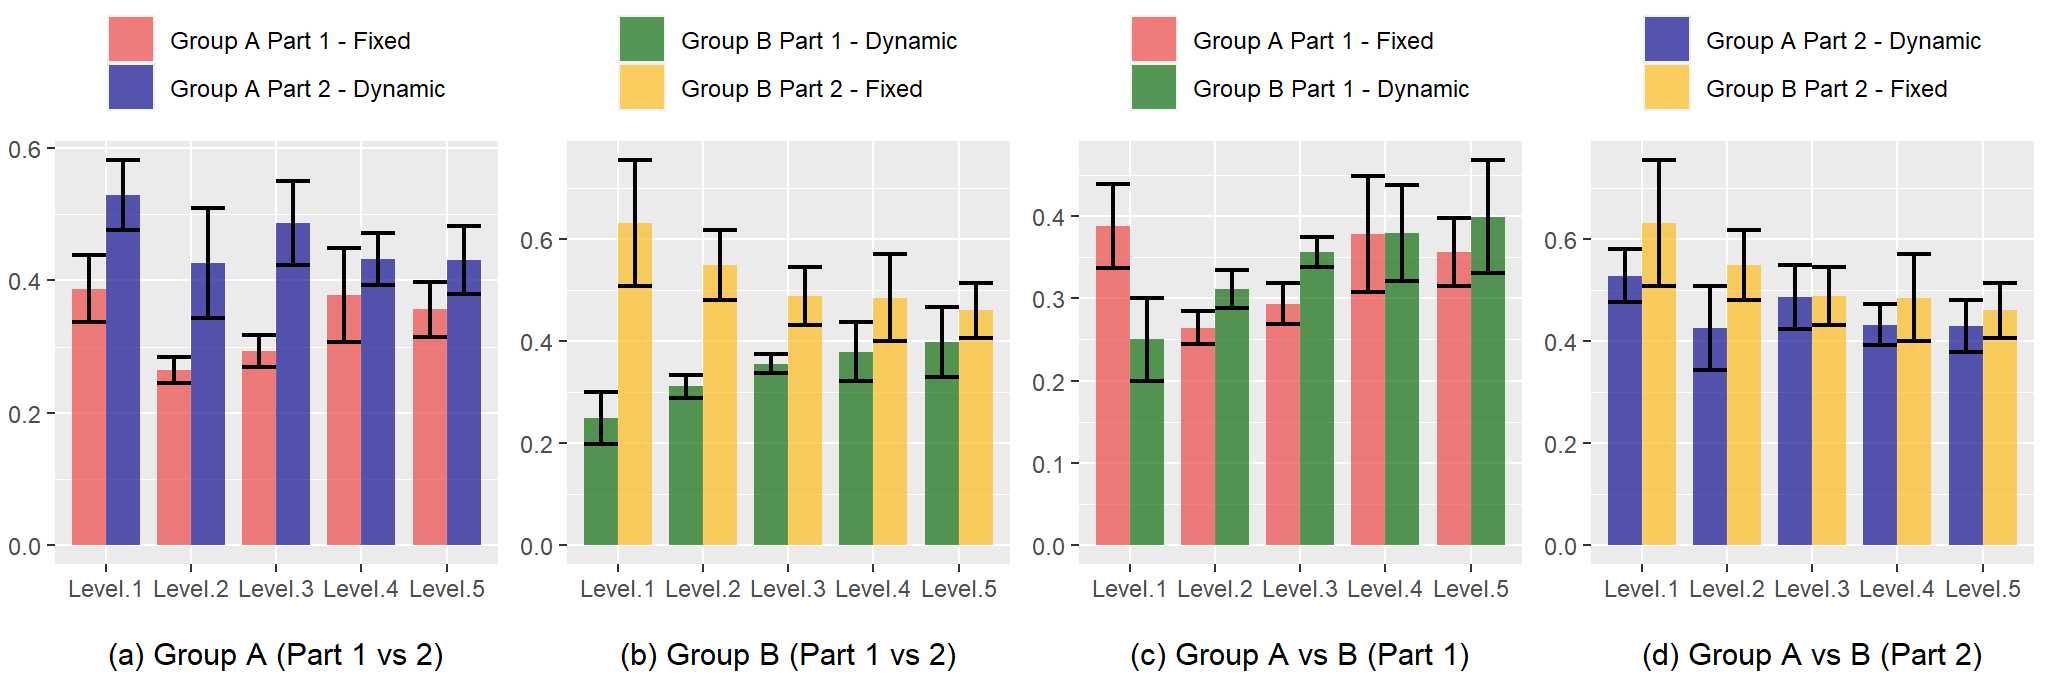
\includegraphics[width=34em]{figures/attack_avoidance_efficiency-beginner_players.png}
        \legend{Source: Assembled by authors.}
        \label{fig:result-metric-beginners-attack-avoidance-efficiency}
    \end{center}
\end{figure}

%attack_window_efficiency
% Avg Attack Window Efficiency per Level - Beginners
% =======================
\begin{figure}[!ht]
    \begin{center}
    \caption{Avg. Attack Window Efficiency (Y) per Level (X) for Beginners.}
        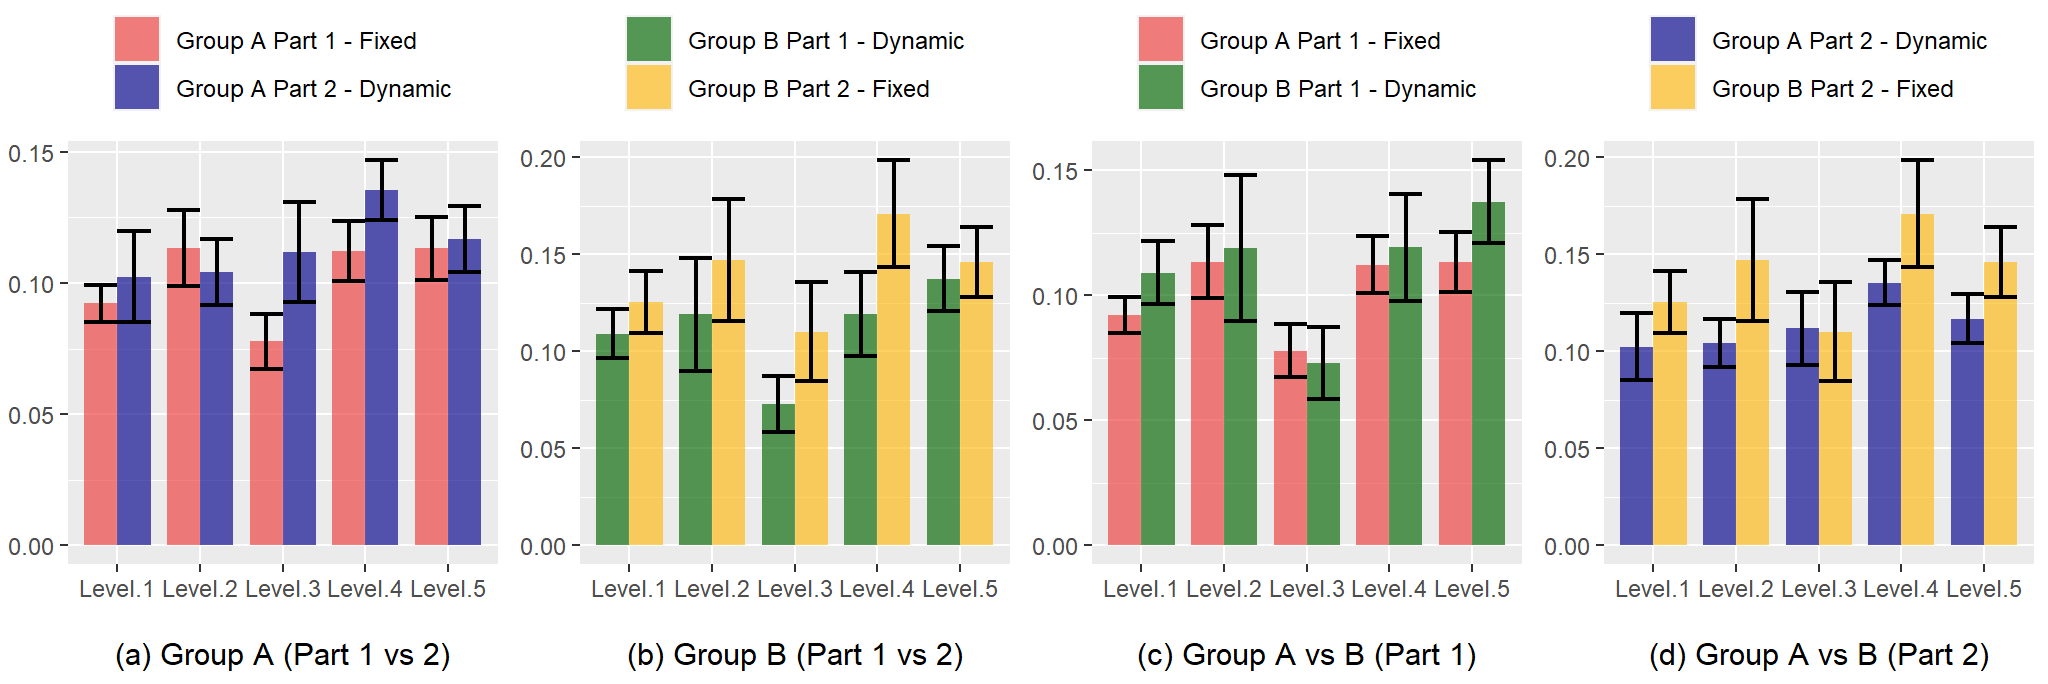
\includegraphics[width=34em]{figures/attack_window_efficiency-beginner_players.png}
        \legend{Source: Assembled by authors.}
        \label{fig:result-metric-beginners-attack-window-efficiency}
    \end{center}
\end{figure}

%completion_time
% Avg Completion Time per Level - Beginners
% =======================
\begin{figure}[!ht]
    \begin{center}
    \caption{Avg. Completion Time (Y) per Level (X) for Beginners.}
        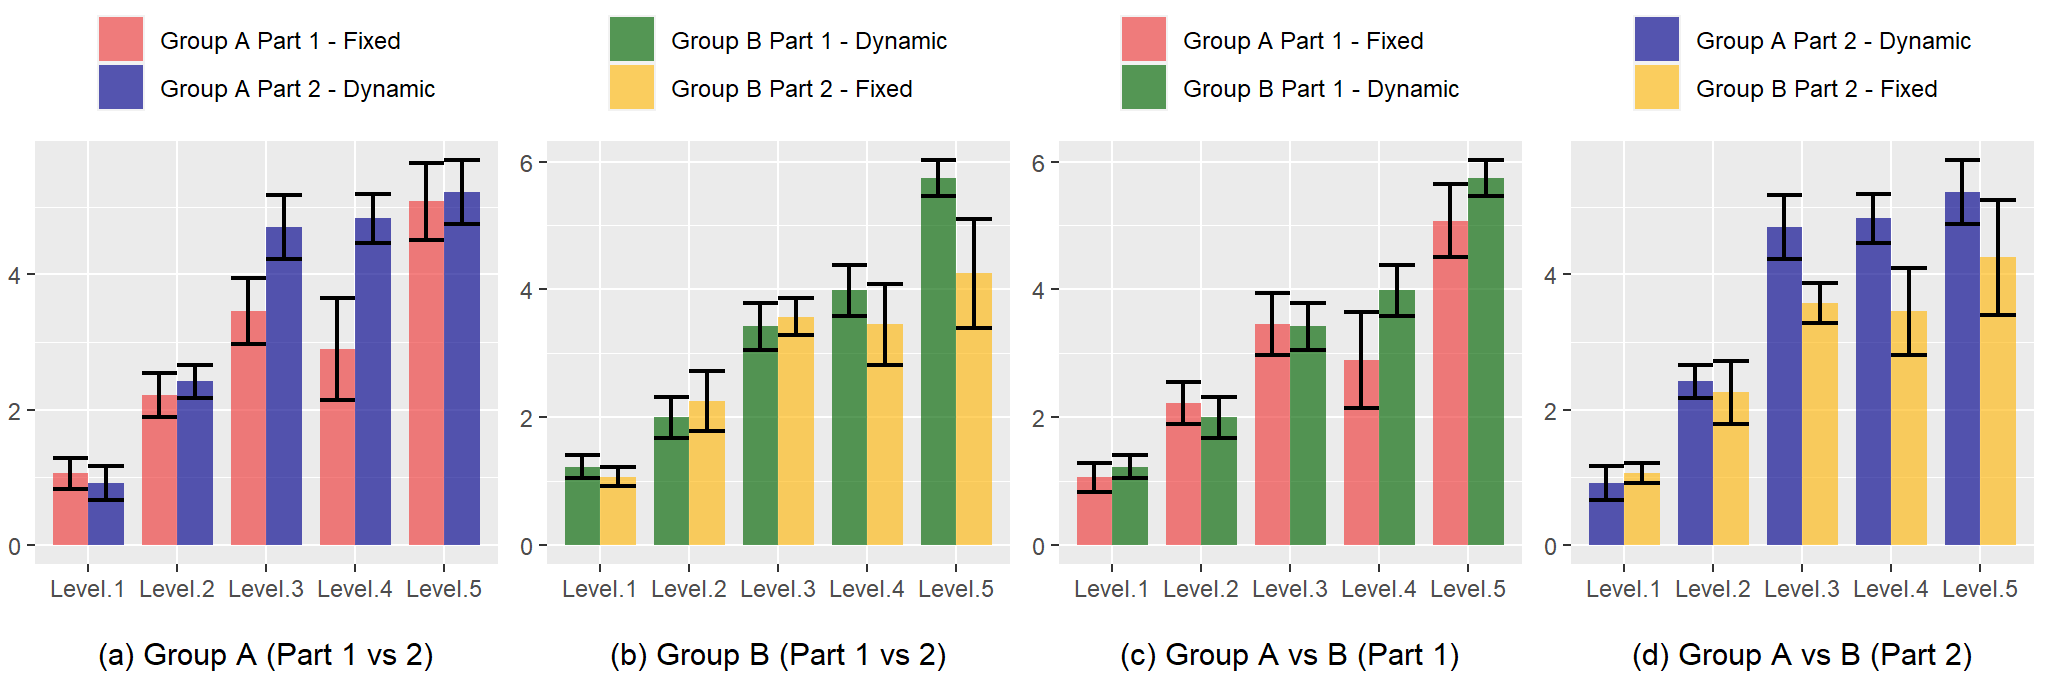
\includegraphics[width=34em]{figures/completion_time-beginner_players.png}
        \legend{Source: Assembled by authors.}
        \label{fig:result-metric-beginners-completion-time}
    \end{center}
\end{figure}

%damage_dealt_per_10s
% Avg Damage Dealt per 10s per Level - Beginners
% =======================
\begin{figure}[!ht]
    \begin{center}
    \caption{Avg. Damage Dealt per 10 seconds (Y) per Level (X) for Beginners.}
        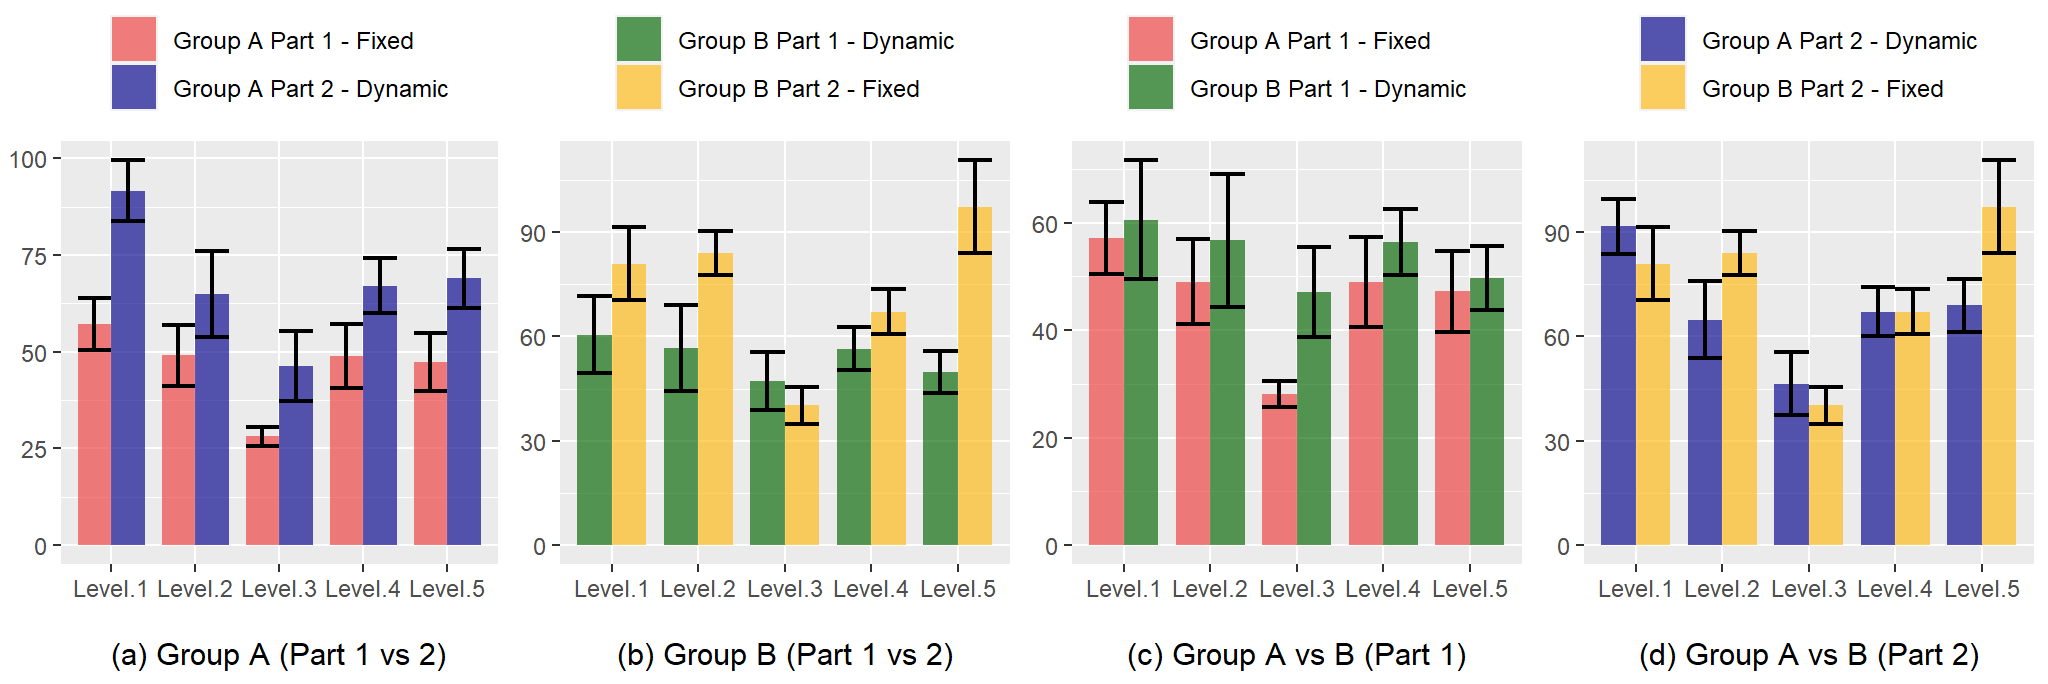
\includegraphics[width=34em]{figures/damage_dealt_per_10s-beginner_players.png}
        \legend{Source: Assembled by authors.}
        \label{fig:result-metric-beginners-damage-dealt-per-10s}
    \end{center}
\end{figure}

%deaths_per_level
% Avg Deaths per Level - Beginners
% =======================
\begin{figure}[!ht]
    \begin{center}
    \caption{Avg. Deaths (Y) per Level (X) for Beginners.}
        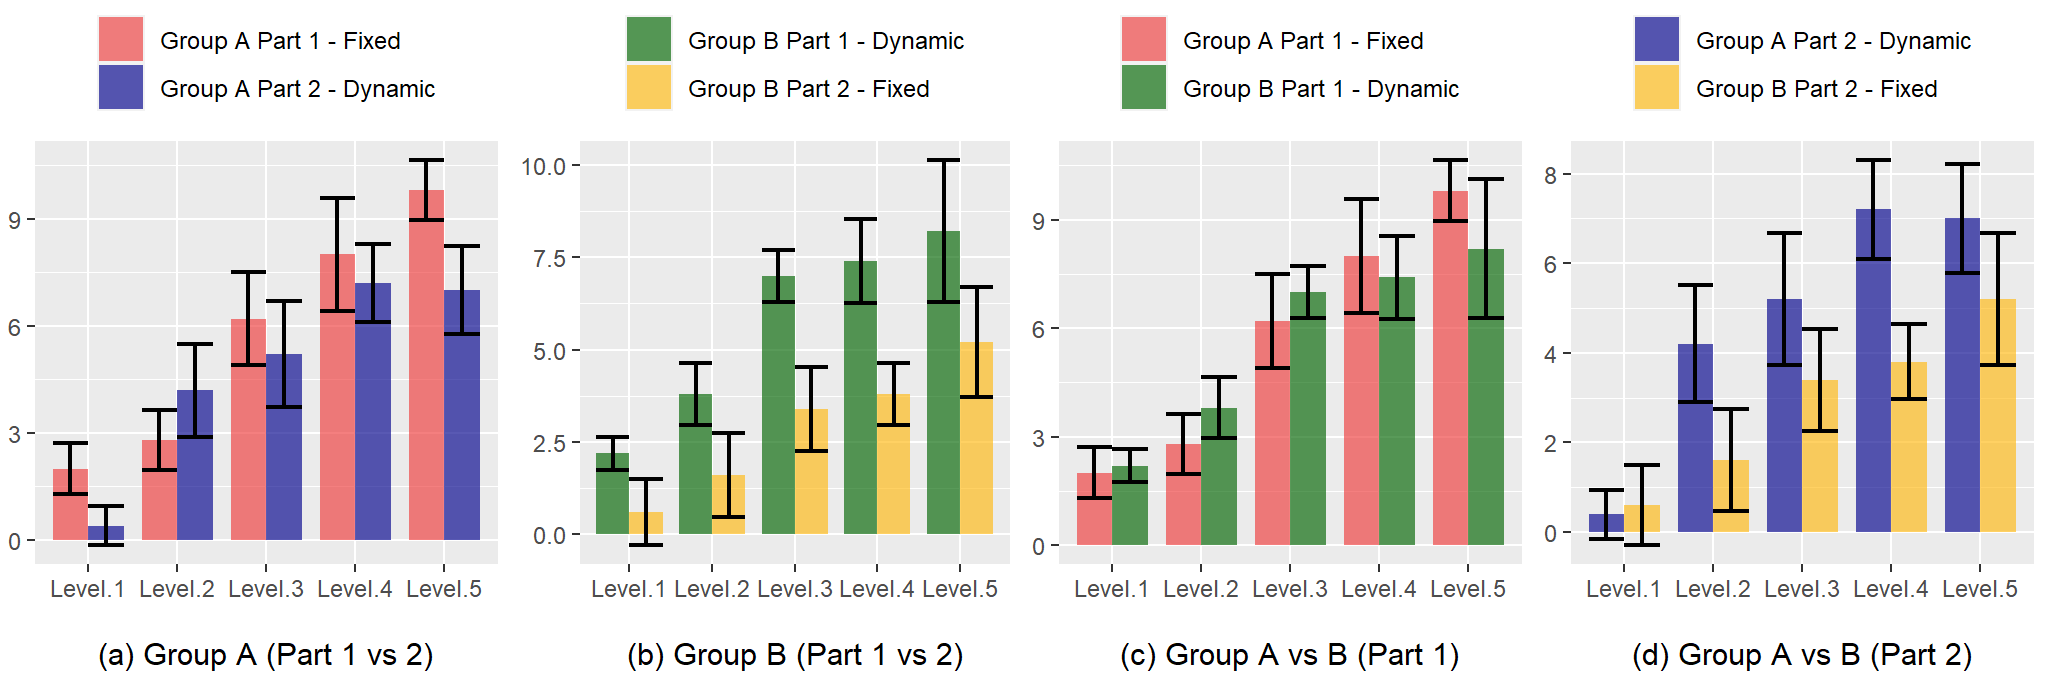
\includegraphics[width=34em]{figures/deaths_per_level-beginner_players.png}
        \legend{Source: Assembled by authors.}
        \label{fig:result-metric-beginners-deaths-per-level}
    \end{center}
\end{figure}

%health_lost_per_encounter
% Avg Health Lost per Encounter per Level - Beginners
% =======================
\begin{figure}[!ht]
    \begin{center}
    \caption{Avg. Health Lost per Encounter (Y) per Level (X) for Beginners.}
        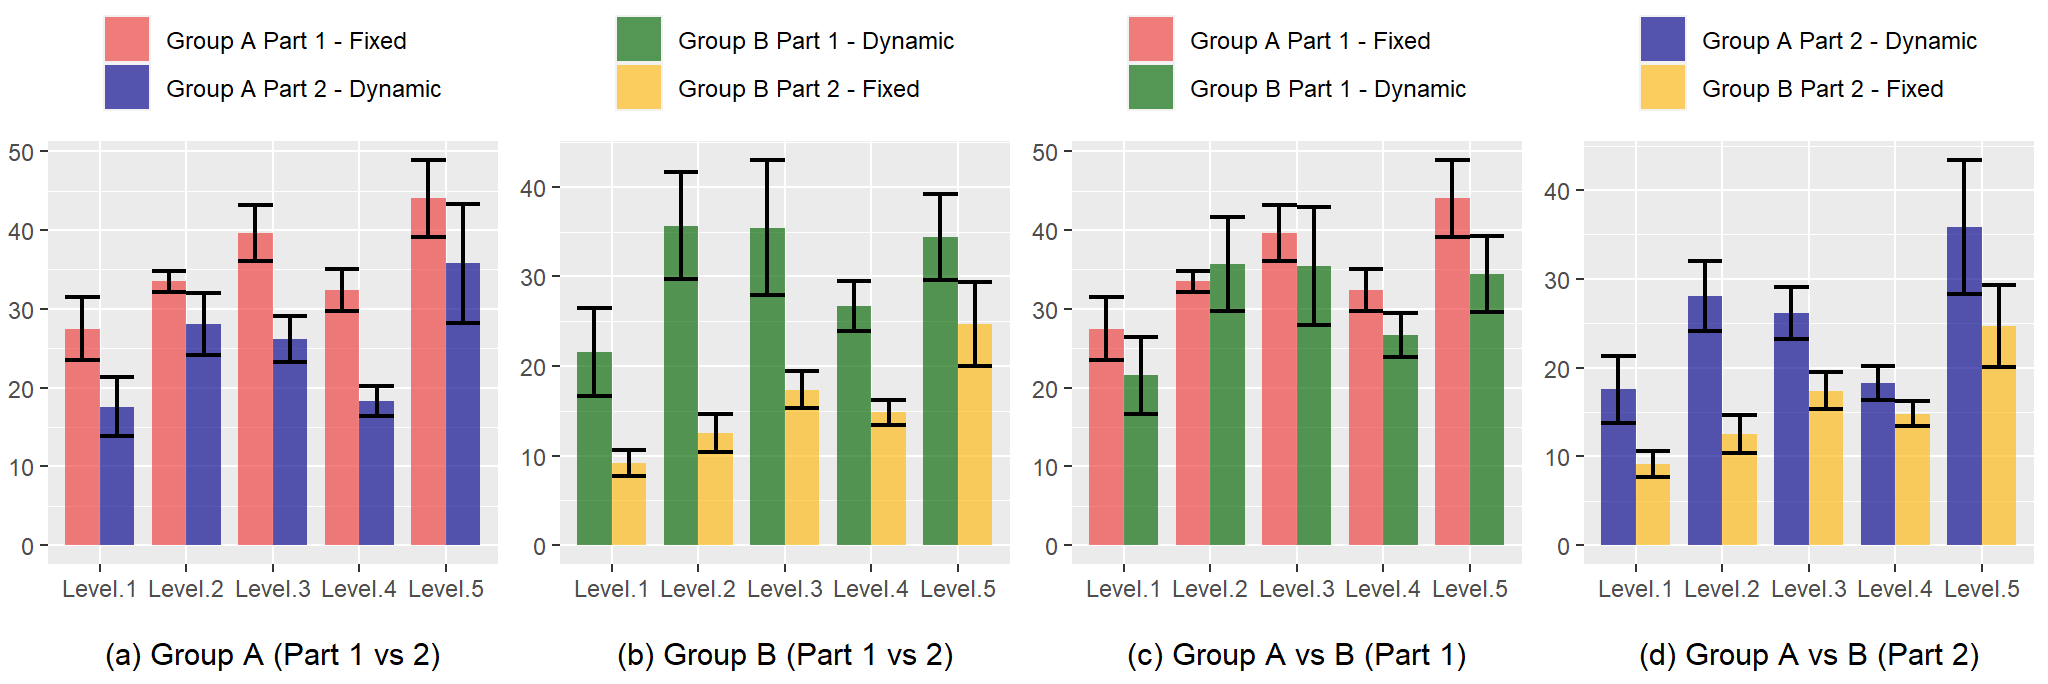
\includegraphics[width=34em]{figures/health_lost_per_encounter-beginner_players.png}
        \legend{Source: Assembled by authors.}
        \label{fig:result-metric-beginners-health-lost-per-encounter}
    \end{center}
\end{figure}

% ==================================================
% ==================================================
% ==================================================

\subsection{Intermediate Players}

% Perception
% =============================

% Performance
% =============================

% Table with Observations for Performance Metrics for Intermediate Players
\begin{table}[!ht]
    \begin{center}
      \caption{Observations on Performance Metrics for Intermediate Players.}
      \label{tab:observations-performance-metrics-intermediates}
      \rowcolors{2}{}{gray!25} % Alternate row colors
      \begin{tabular}{ w{c}{6em} m{27em} } % alignments and column size
        \addlinespace
        \toprule
        % Headings
        \bf Metric & \bf Observations  \\
        \midrule
        % Data
        \makecell[c]{Adjustment\\Target} & \\
        \makecell[c]{Attack\\Avoidance\\Efficiency} & \\
        \makecell[c]{Attack\\Window\\Efficiency} & \\
        \makecell[c]{Completion\\Time} & \\
        \makecell[c]{Damage Dealt\\per 10 seconds} & \\
        \makecell[c]{Deaths per\\Level} & \\
        \makecell[c]{Health Lost\\per Encounter} & \\
        \bottomrule
      \end{tabular}
    \end{center}
\end{table}

%adjustment_target_level
% Avg Adjustment Target per Level - Intermediates
% =======================
\begin{figure}[!ht]
    \begin{center}
    \caption{Avg. Adjustment Target (Y) per Level (X) for Intermediates.}
        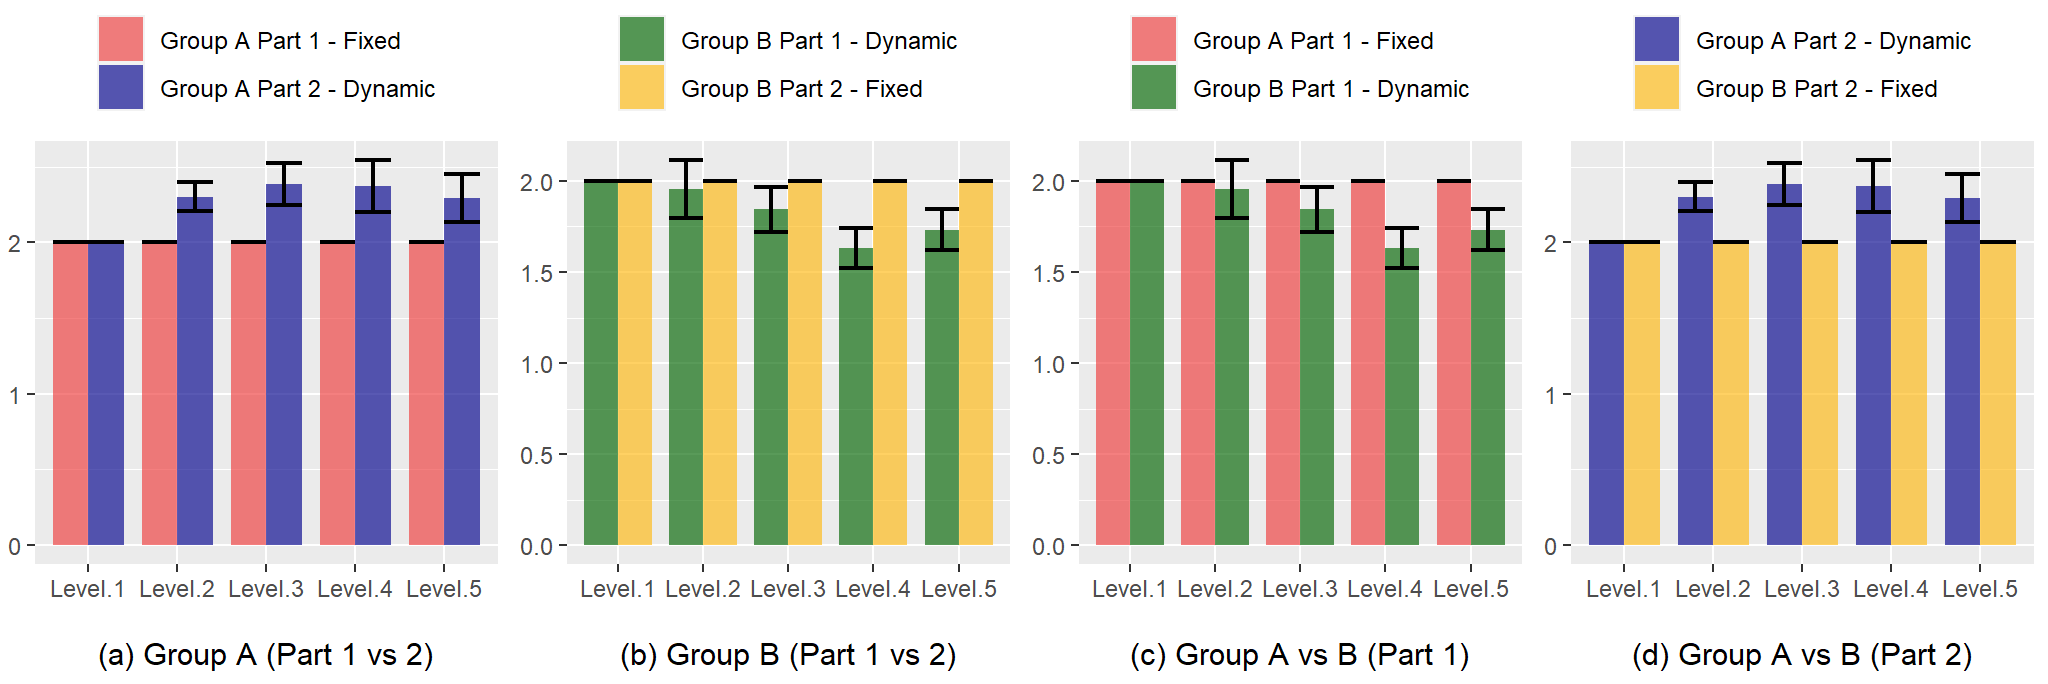
\includegraphics[width=34em]{figures/adjustment_target_level-intermediate_players.png}
        \legend{Source: Assembled by authors.}
        \label{fig:result-metric-intermediate-adjustment-target-level}
    \end{center}
\end{figure}

%attack_avoidance_efficiency
% Avg Attack Avoidance Efficiency per Level - Intermediates
% =======================
\begin{figure}[!ht]
    \begin{center}
    \caption{Avg. Attack Avoidance Efficiency (Y) per Level (X) for Intermediates.}
        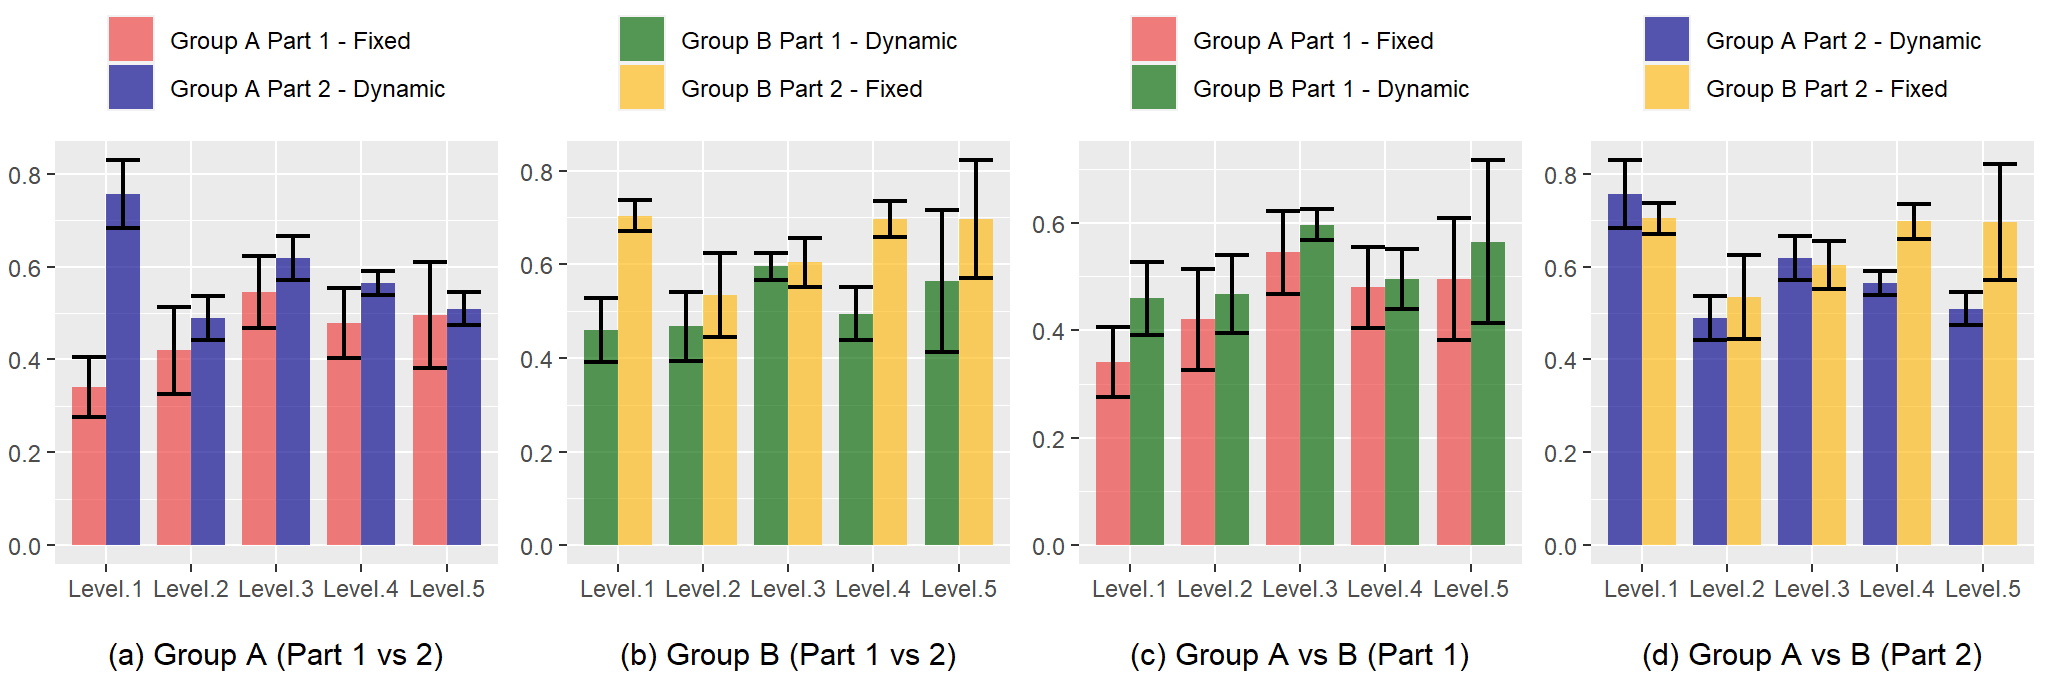
\includegraphics[width=34em]{figures/attack_avoidance_efficiency-intermediate_players.png}
        \legend{Source: Assembled by authors.}
        \label{fig:result-metric-intermediates-attack-avoidance-efficiency}
    \end{center}
\end{figure}

%attack_window_efficiency
% Avg Attack Window Efficiency per Level - Intermediates
% =======================
\begin{figure}[!ht]
    \begin{center}
    \caption{Avg. Attack Window Efficiency (Y) per Level (X) for Intermediates.}
        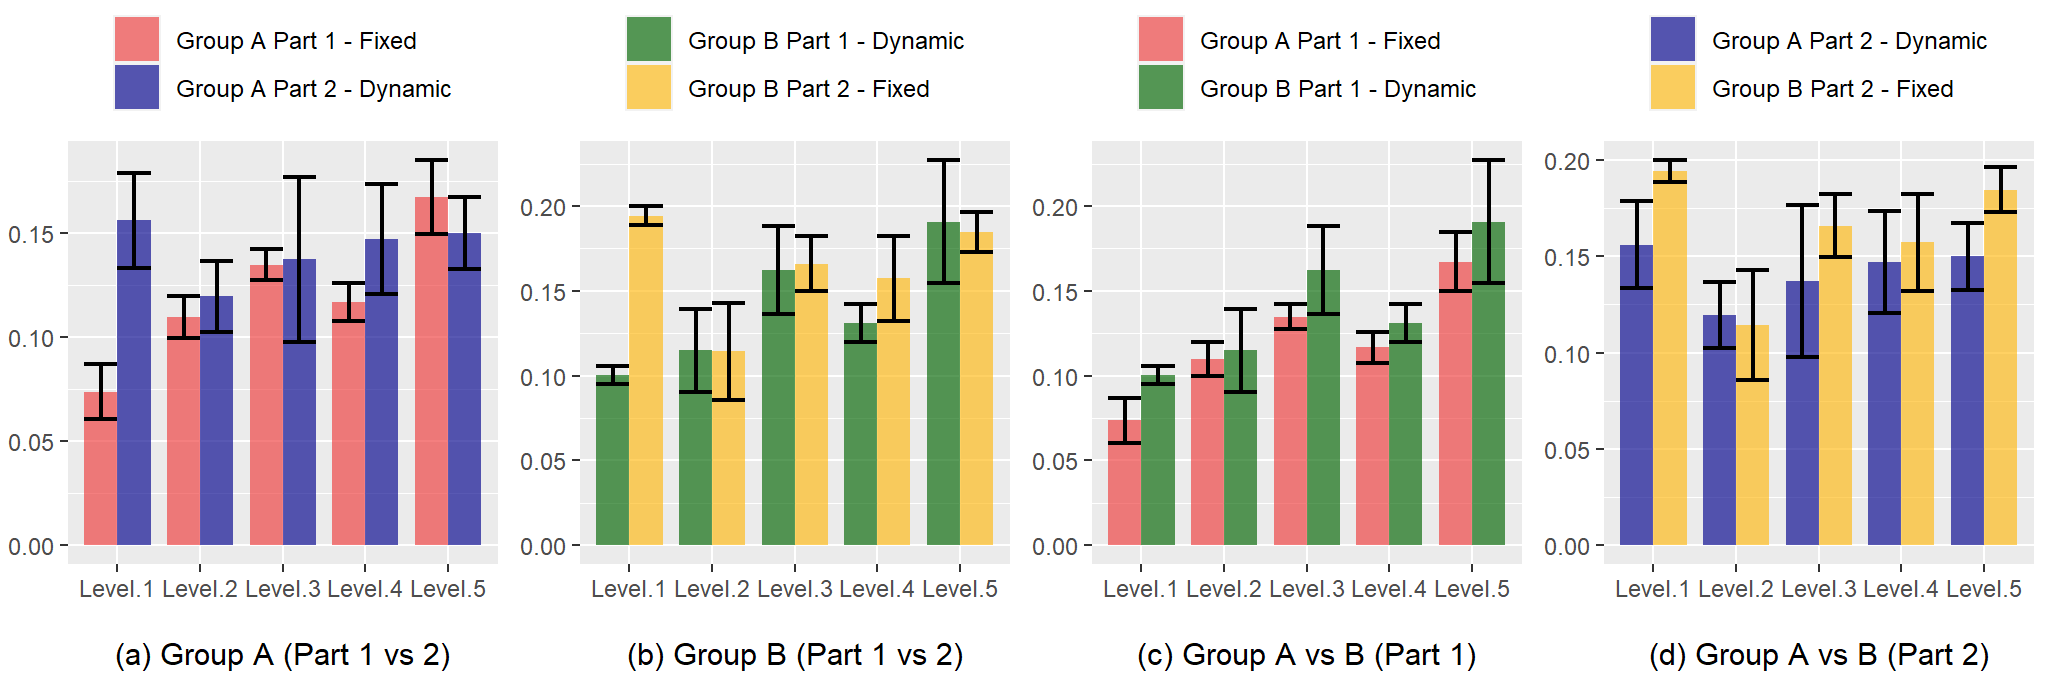
\includegraphics[width=34em]{figures/attack_window_efficiency-intermediate_players.png}
        \legend{Source: Assembled by authors.}
        \label{fig:result-metric-intermediates-attack-window-efficiency}
    \end{center}
\end{figure}

%completion_time
% Avg Completion Time per Level - Intermediates
% =======================
\begin{figure}[!ht]
    \begin{center}
    \caption{Avg. Completion Time (Y) per Level (X) for Intermediates.}
        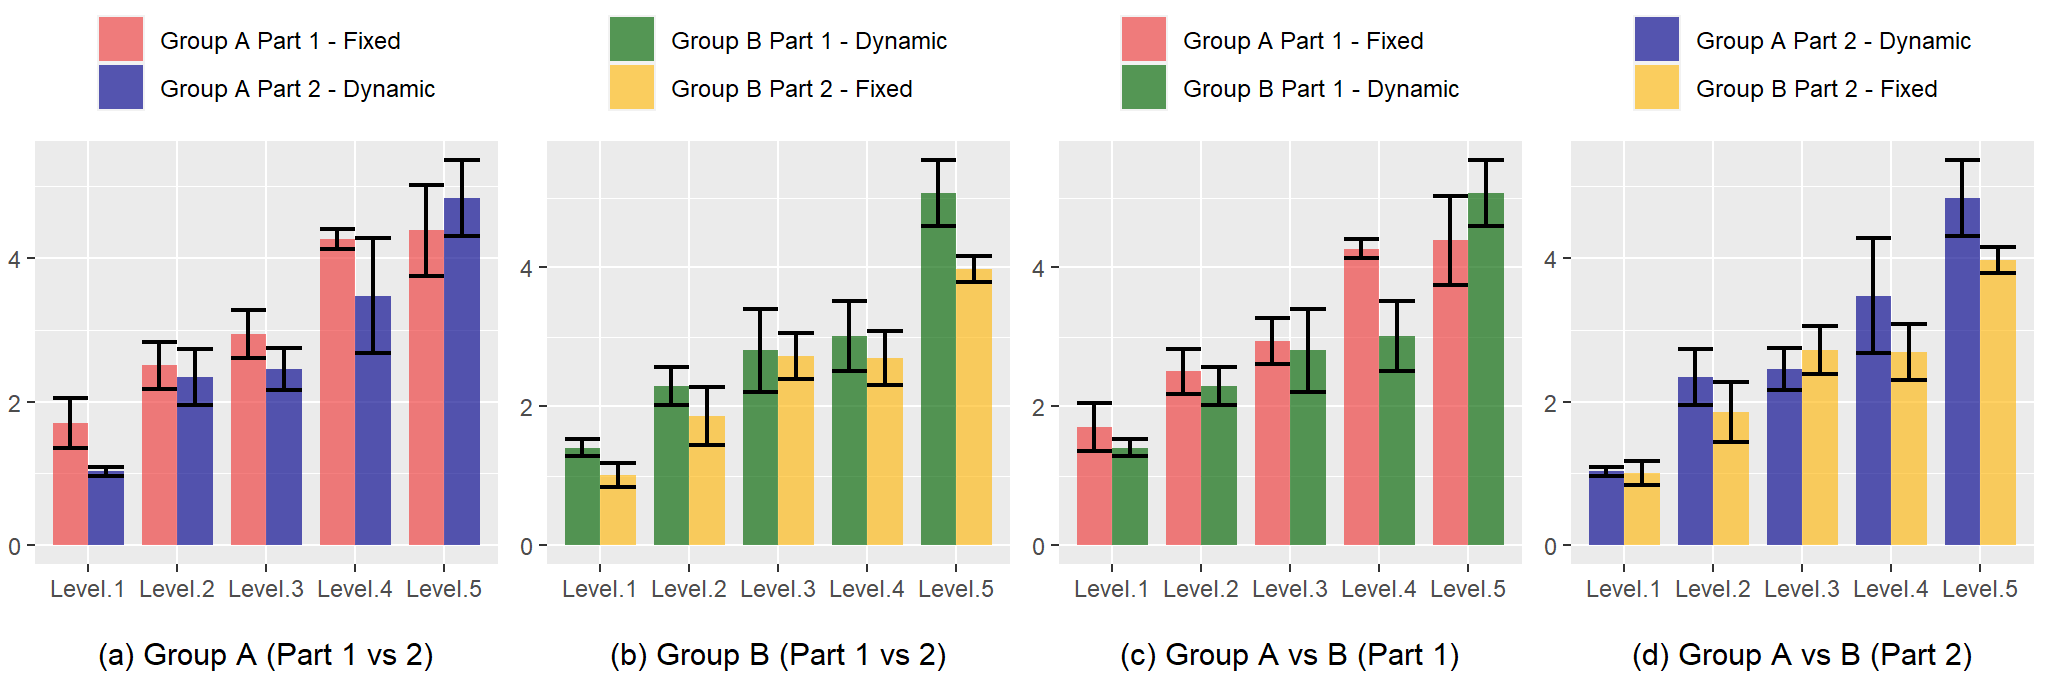
\includegraphics[width=34em]{figures/completion_time-intermediate_players.png}
        \legend{Source: Assembled by authors.}
        \label{fig:result-metric-intermediates-completion-time}
    \end{center}
\end{figure}

%damage_dealt_per_10s
% Avg Damage Dealt per 10s per Level - Intermediates
% =======================
\begin{figure}[!ht]
    \begin{center}
    \caption{Avg. Damage Dealt per 10 seconds (Y) per Level (X) for Intermediates.}
        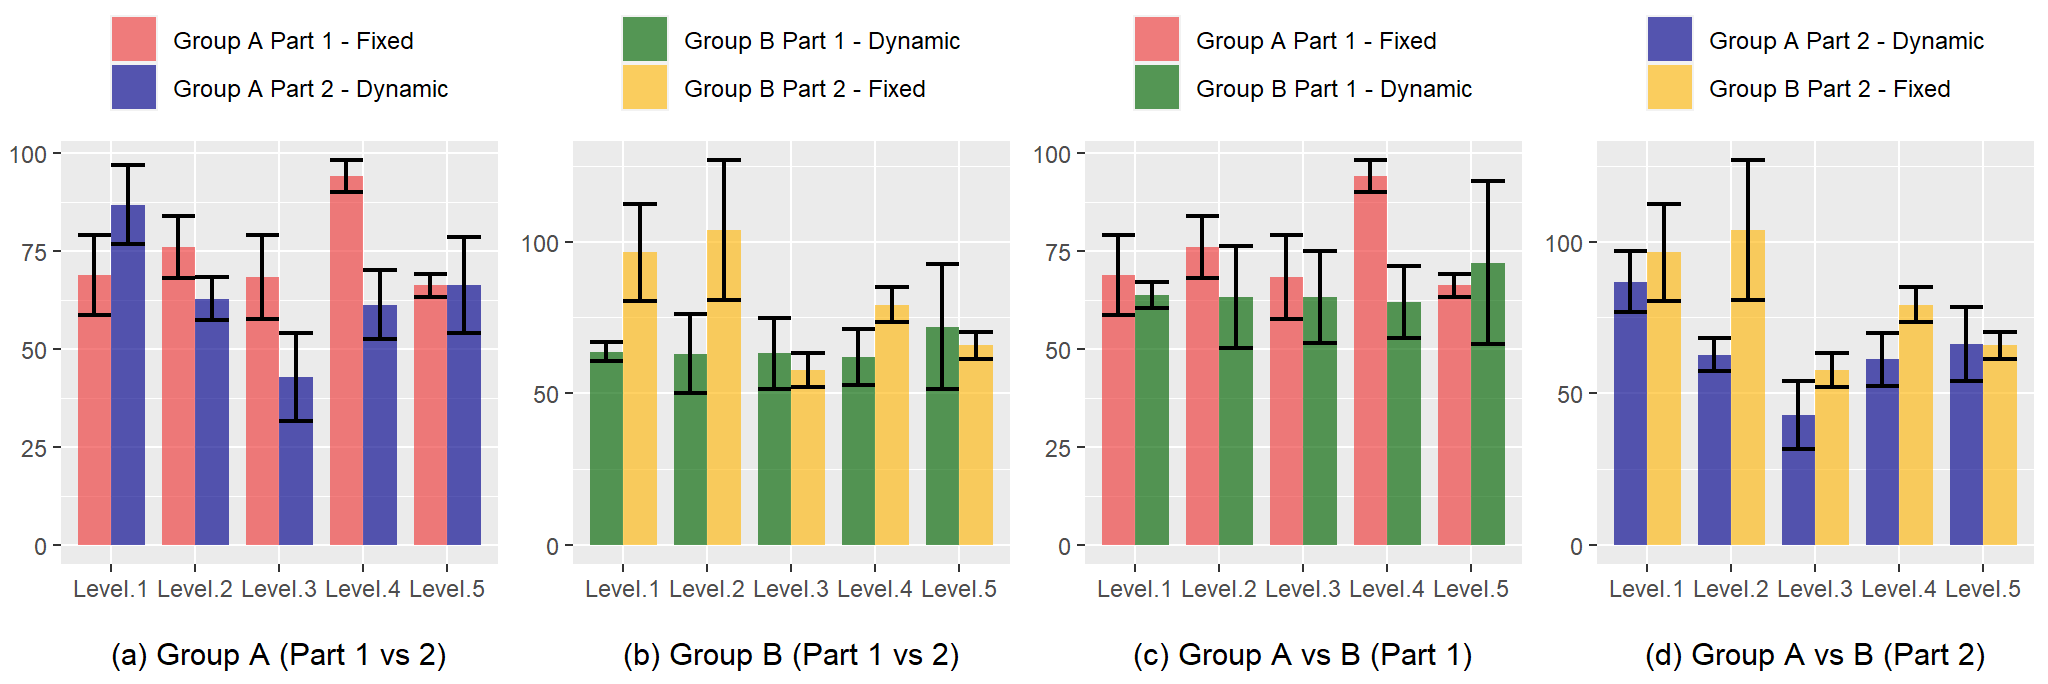
\includegraphics[width=34em]{figures/damage_dealt_per_10s-intermediate_players.png}
        \legend{Source: Assembled by authors.}
        \label{fig:result-metric-intermediates-damage-dealt-per-10s}
    \end{center}
\end{figure}

%deaths_per_level
% Avg Deaths per Level - Intermediates
% =======================
\begin{figure}[!ht]
    \begin{center}
    \caption{Avg. Deaths (Y) per Level (X) for Intermediates.}
        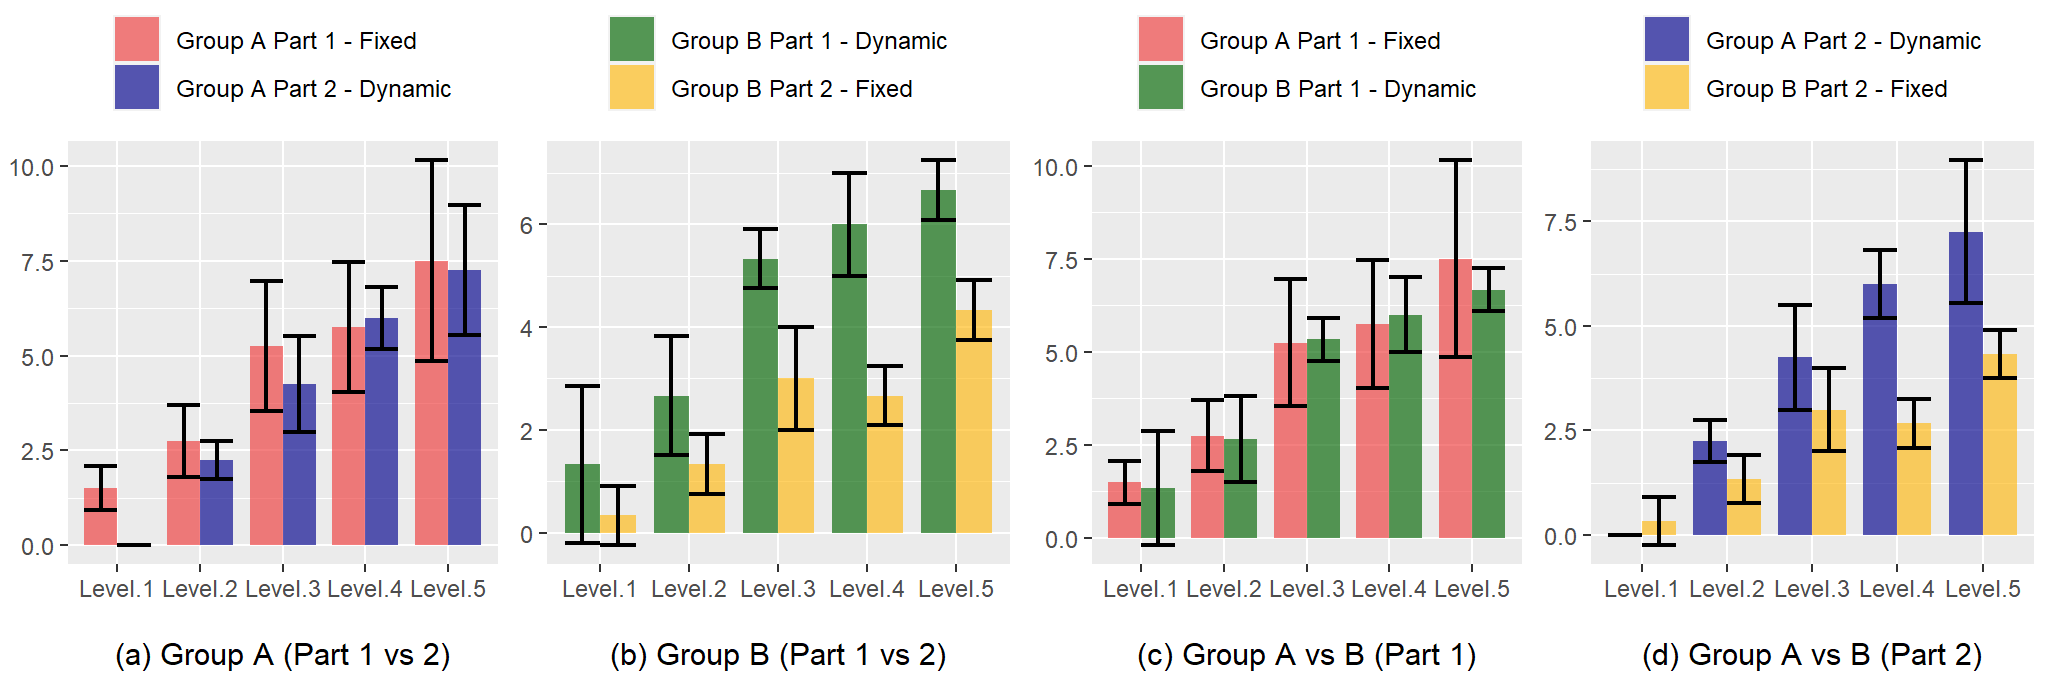
\includegraphics[width=34em]{figures/deaths_per_level-intermediate_players.png}
        \legend{Source: Assembled by authors.}
        \label{fig:result-metric-intermediates-deaths-per-level}
    \end{center}
\end{figure}

%health_lost_per_encounter
% Avg Health Lost per Encounter per Level - Intermediates
% =======================
\begin{figure}[!ht]
    \begin{center}
    \caption{Avg. Health Lost per Encounter (Y) per Level (X) for Intermediates.}
        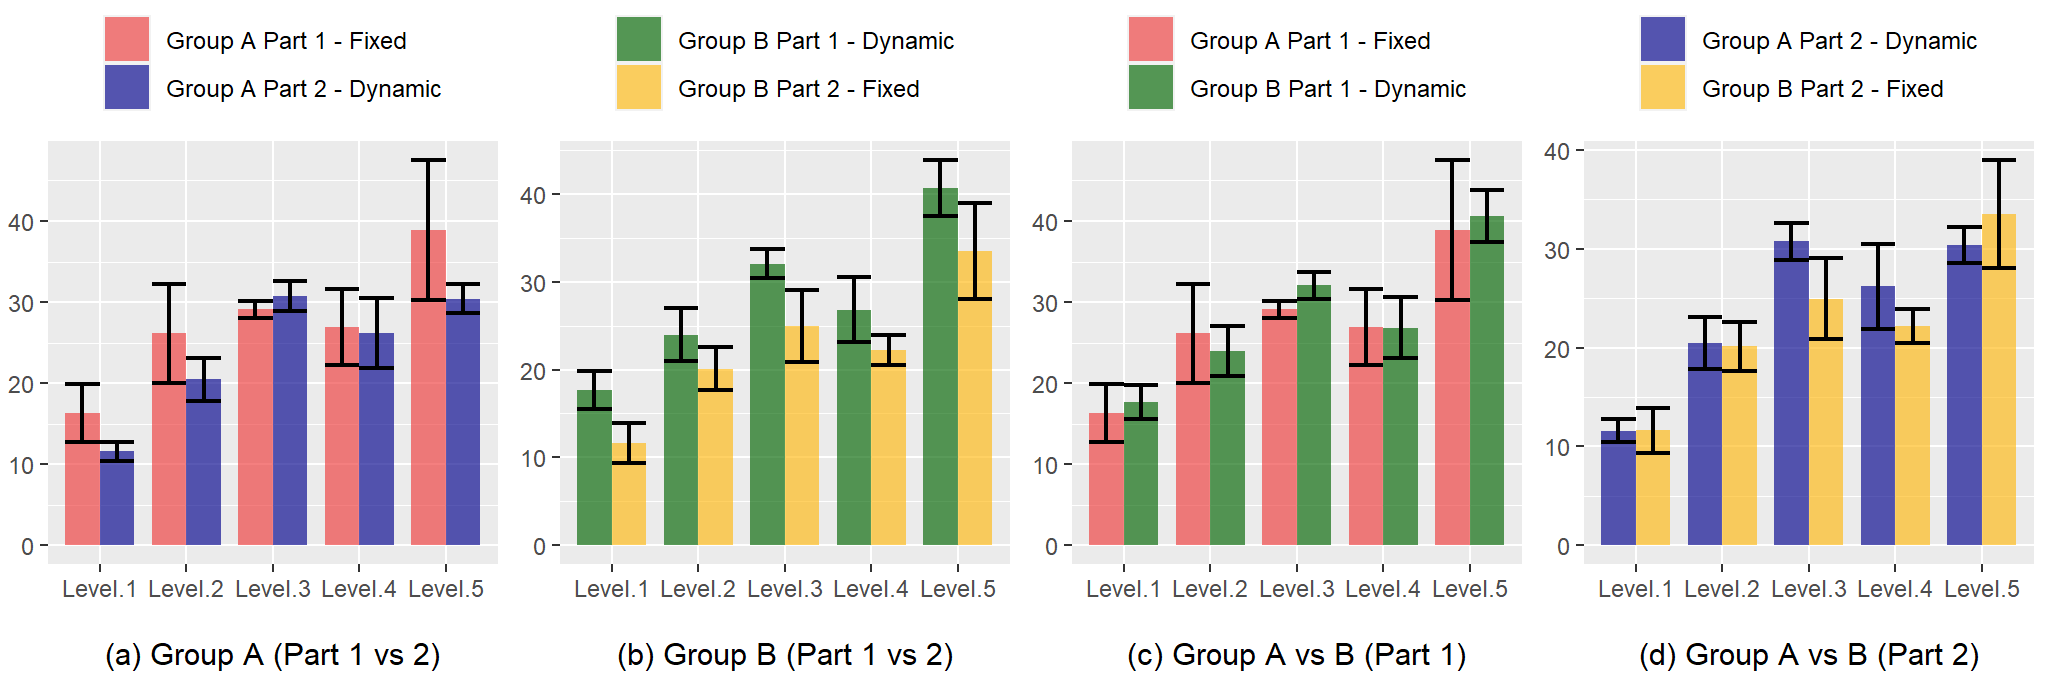
\includegraphics[width=34em]{figures/health_lost_per_encounter-intermediate_players.png}
        \legend{Source: Assembled by authors.}
        \label{fig:result-metric-intermediates-health-lost-per-encounter}
    \end{center}
\end{figure}

% ==================================================
% ==================================================
% ==================================================

\subsection{Veteran Players}

% Perception
% =============================

% Performance
% =============================

% Table with Observations for Performance Metrics for Veteran Players
\begin{table}[!ht]
    \begin{center}
      \caption{Observations on Performance Metrics for Veteran Players.}
      \label{tab:observations-performance-metrics-veterans}
      \rowcolors{2}{}{gray!25} % Alternate row colors
      \begin{tabular}{ w{c}{6em} m{27em} } % alignments and column size
        \addlinespace
        \toprule
        % Headings
        \bf Metric & \bf Observations  \\
        \midrule
        % Data
        \makecell[c]{Adjustment\\Target} & \\
        \makecell[c]{Attack\\Avoidance\\Efficiency} & \\
        \makecell[c]{Attack\\Window\\Efficiency} & \\
        \makecell[c]{Completion\\Time} & \\
        \makecell[c]{Damage Dealt\\per 10 seconds} & \\
        \makecell[c]{Deaths per\\Level} & \\
        \makecell[c]{Health Lost\\per Encounter} & \\
        \bottomrule
      \end{tabular}
    \end{center}
\end{table}

%adjustment_target_level
% Avg Adjustment Target per Level - Veterans
% =======================
\begin{figure}[!ht]
    \begin{center}
    \caption{Avg. Adjustment Target (Y) per Level (X) for Veterans.}
        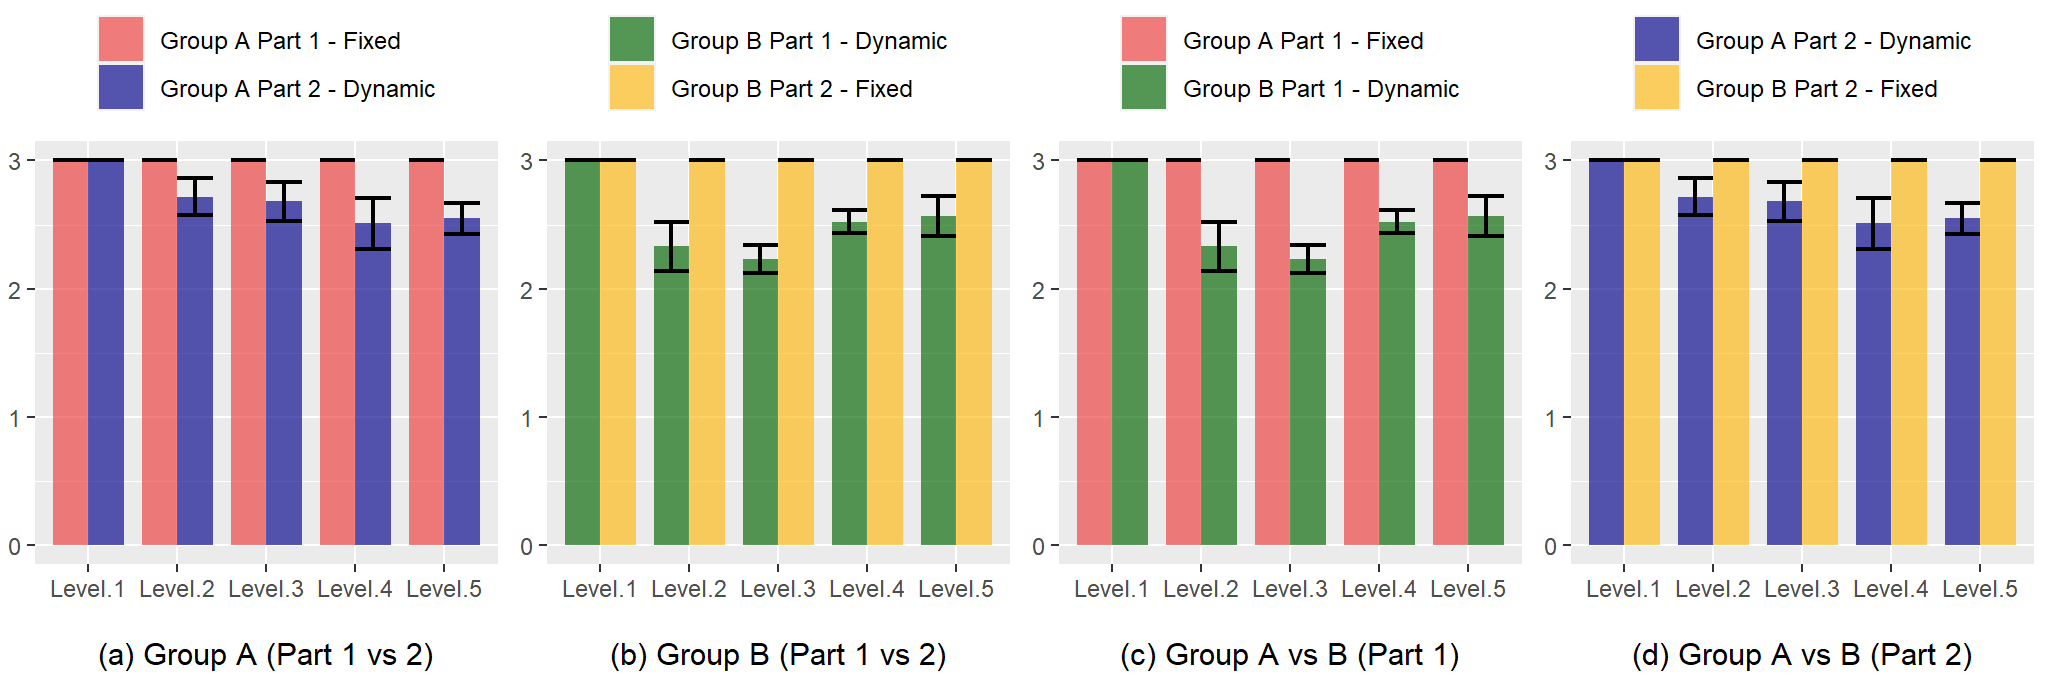
\includegraphics[width=34em]{figures/adjustment_target_level-veteran_players.png}
    \legend{Source: Assembled by authors.}
    \label{fig:result-metric-veteran-adjustment-target-level}
    \end{center}
\end{figure}

%attack_avoidance_efficiency
% Avg Attack Avoidance Efficiency per Level - Veterans
% =======================
\begin{figure}[!ht]
    \begin{center}
        \caption{Avg. Attack Avoidance Efficiency (Y) per Level (X) for Veterans.}
        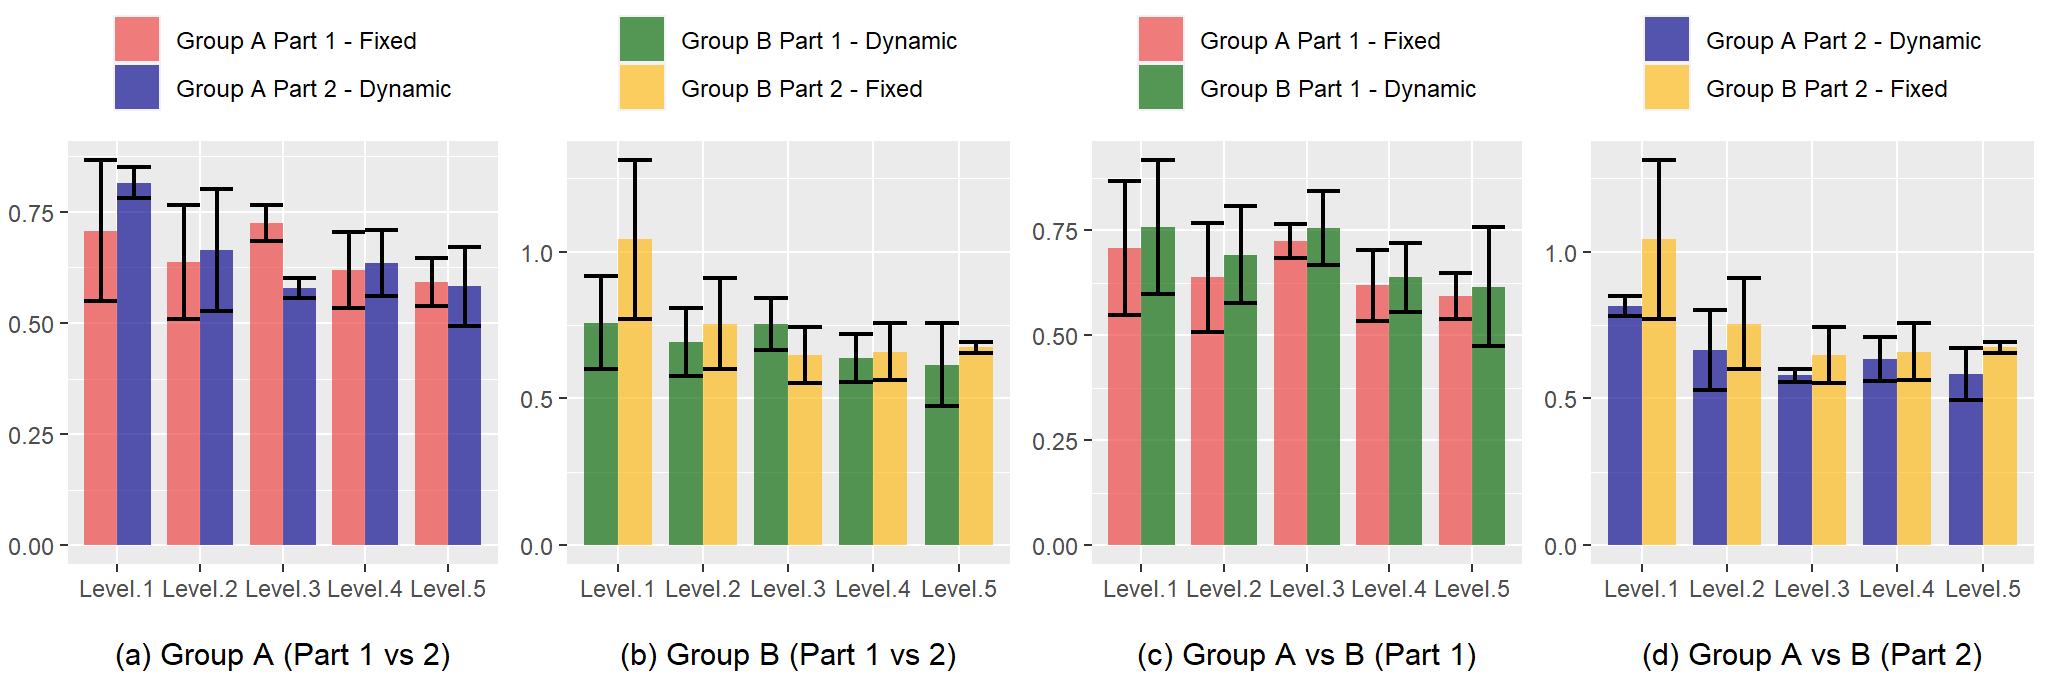
\includegraphics[width=34em]{figures/attack_avoidance_efficiency-veteran_players.png}
    \legend{Source: Assembled by authors.}
    \label{fig:result-metric-veterans-attack-avoidance-efficiency}
    \end{center}
\end{figure}

%attack_window_efficiency
% Avg Attack Window Efficiency per Level - Veterans
% =======================
\begin{figure}[!ht]
    \begin{center}
    \caption{Avg. Attack Window Efficiency (Y) per Level (X) for Veterans.}
        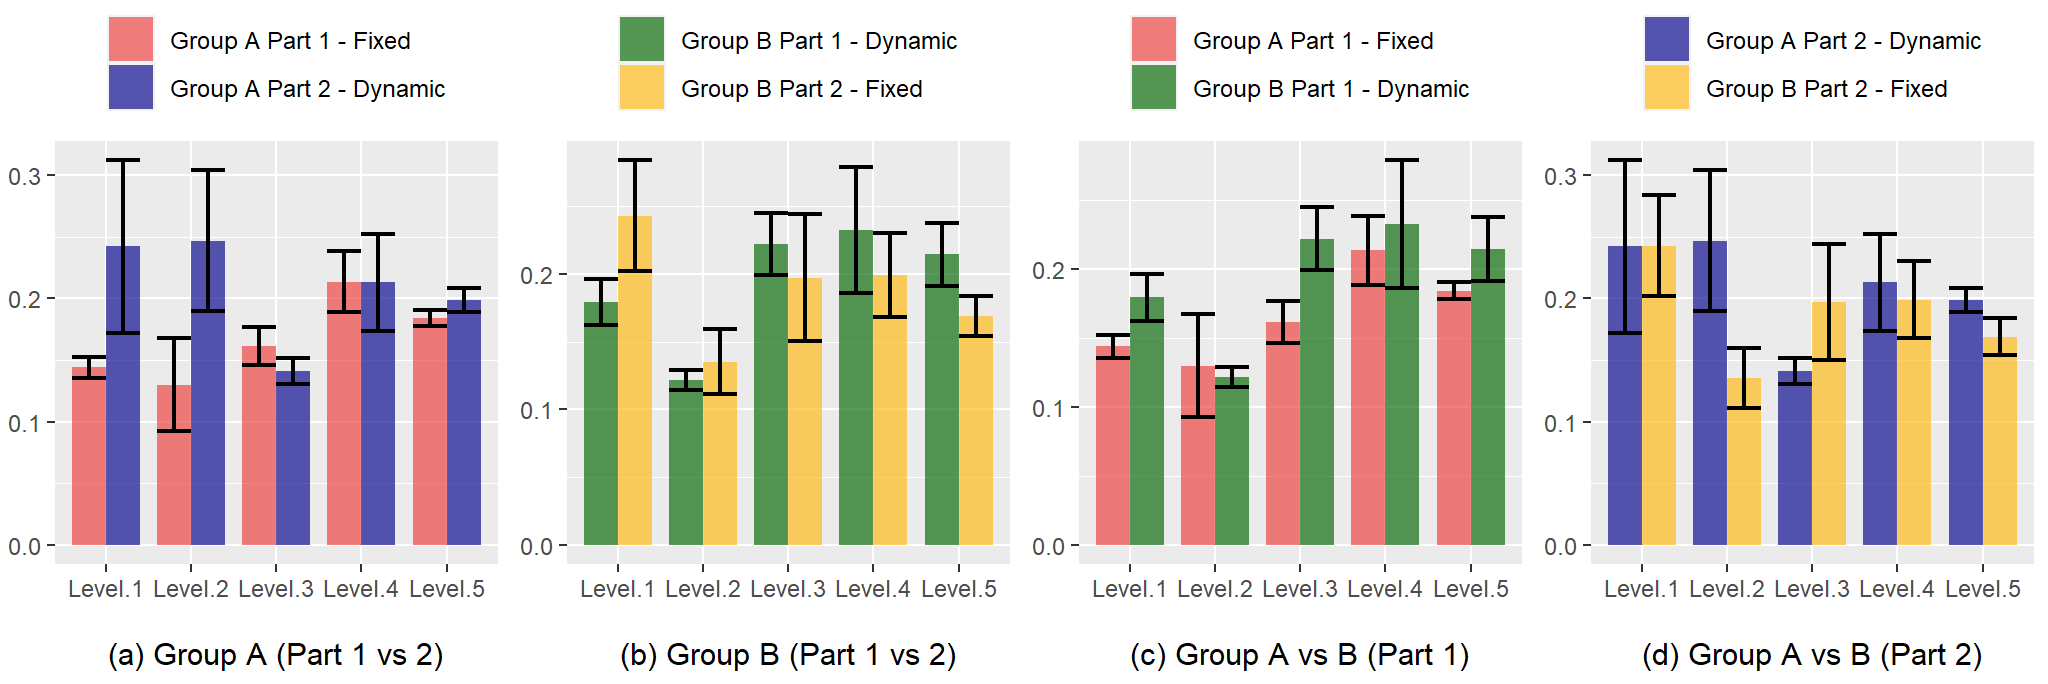
\includegraphics[width=34em]{figures/attack_window_efficiency-veteran_players.png}
    \legend{Source: Assembled by authors.}
    \label{fig:result-metric-veterans-attack-window-efficiency}
    \end{center}
\end{figure}

%completion_time
% Avg Completion Time per Level - Veterans
% =======================
\begin{figure}[!ht]
    \begin{center}
    \caption{Avg. Completion Time (Y) per Level (X) for Veterans.}
        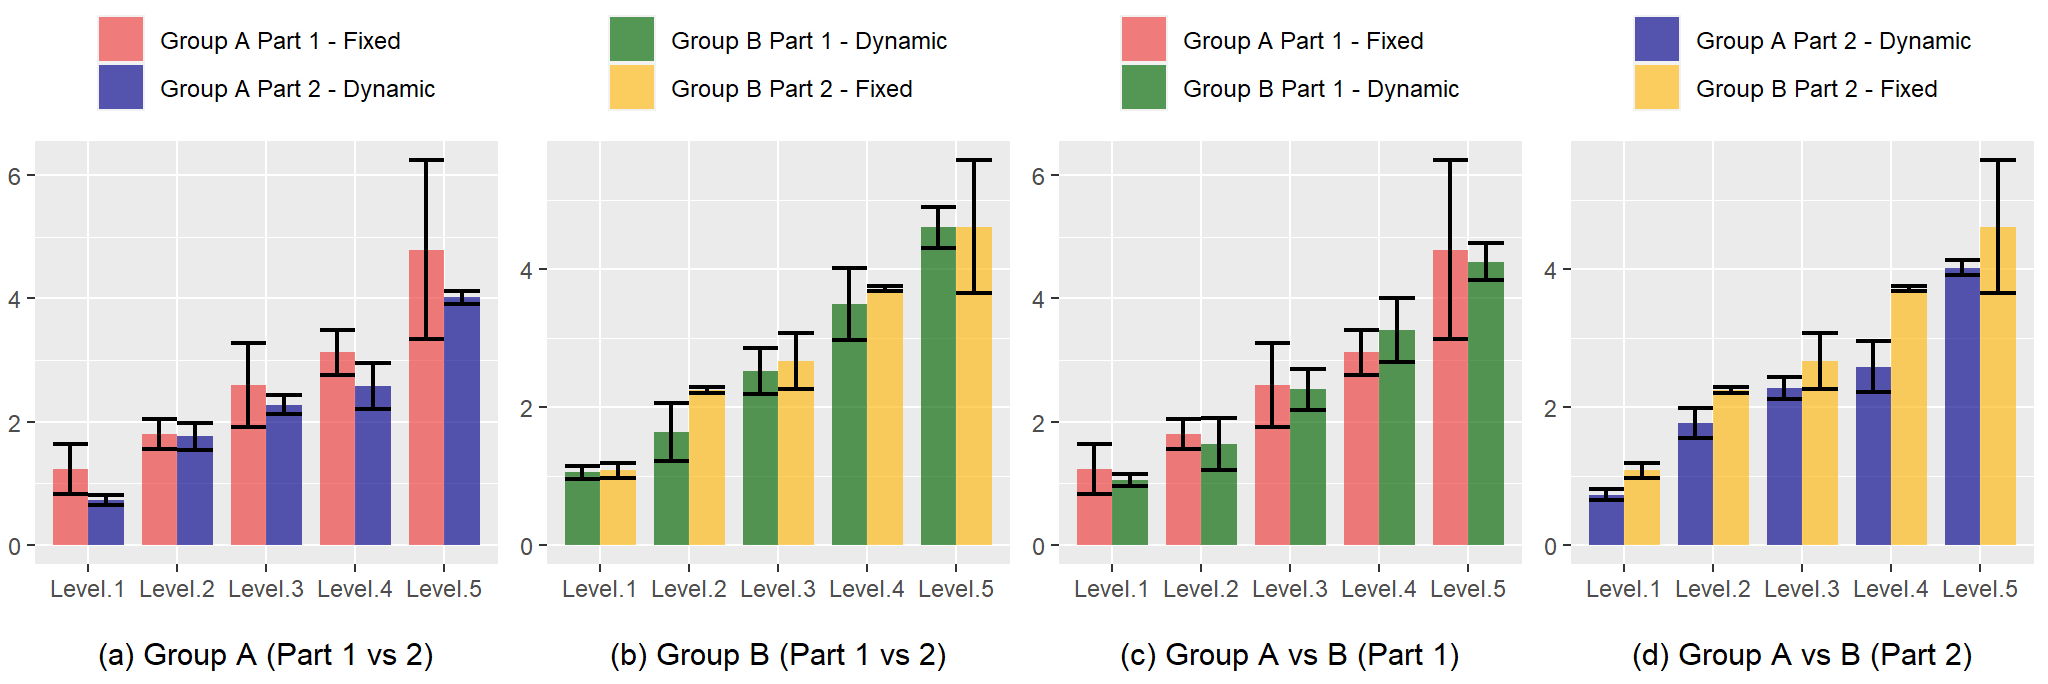
\includegraphics[width=34em]{figures/completion_time-veteran_players.png}
        \legend{Source: Assembled by authors.}
        \label{fig:result-metric-veterans-completion-time}
    \end{center}
\end{figure}

%damage_dealt_per_10s
% Avg Damage Dealt per 10s per Level - Veterans
% =======================
\begin{figure}[!ht]
    \begin{center}
    \caption{Avg. Damage Dealt per 10 seconds (Y) per Level (X) for Veterans.}
        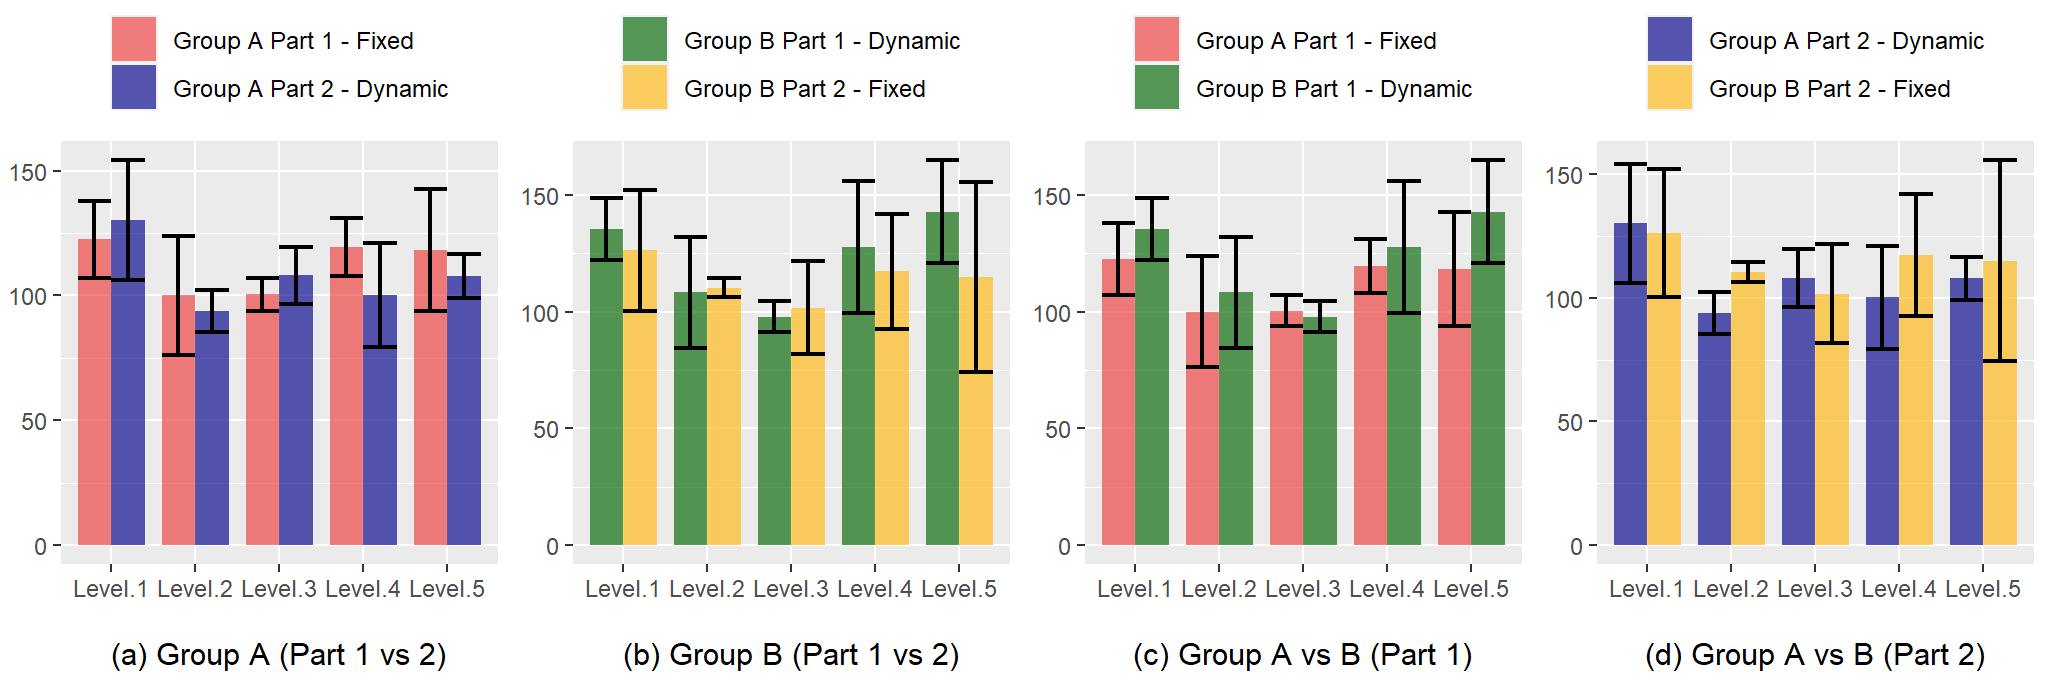
\includegraphics[width=34em]{figures/damage_dealt_per_10s-veteran_players.png}
        \legend{Source: Assembled by authors.}
        \label{fig:result-metric-veterans-damage-dealt-per-10s}
    \end{center}
\end{figure}

%deaths_per_level
% Avg Deaths per Level - Veterans
% =======================
\begin{figure}[!ht]
    \begin{center}
    \caption{Avg. Deaths (Y) per Level (X) for Veterans.}
        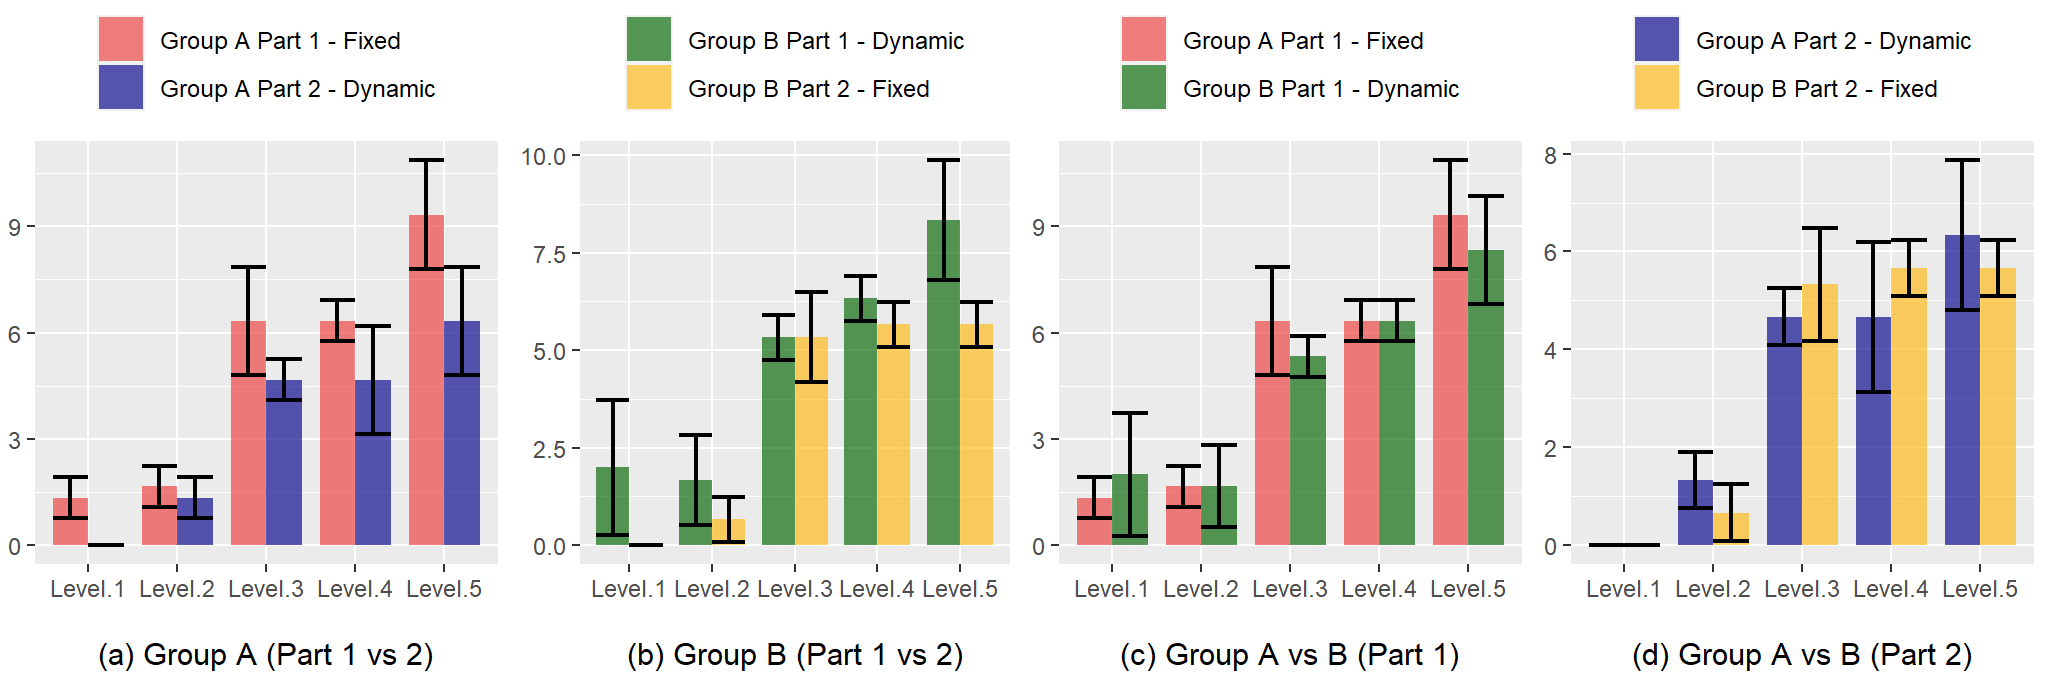
\includegraphics[width=34em]{figures/deaths_per_level-veteran_players.png}
        \legend{Source: Assembled by authors.}
        \label{fig:result-metric-veterans-deaths-per-level}
    \end{center}
\end{figure}

%health_lost_per_encounter
% Avg Health Lost per Encounter per Level - Veterans
% =======================
\begin{figure}[!ht]
    \begin{center}
    \caption{Avg. Health Lost per Encounter (Y) per Level (X) for Veterans.}
        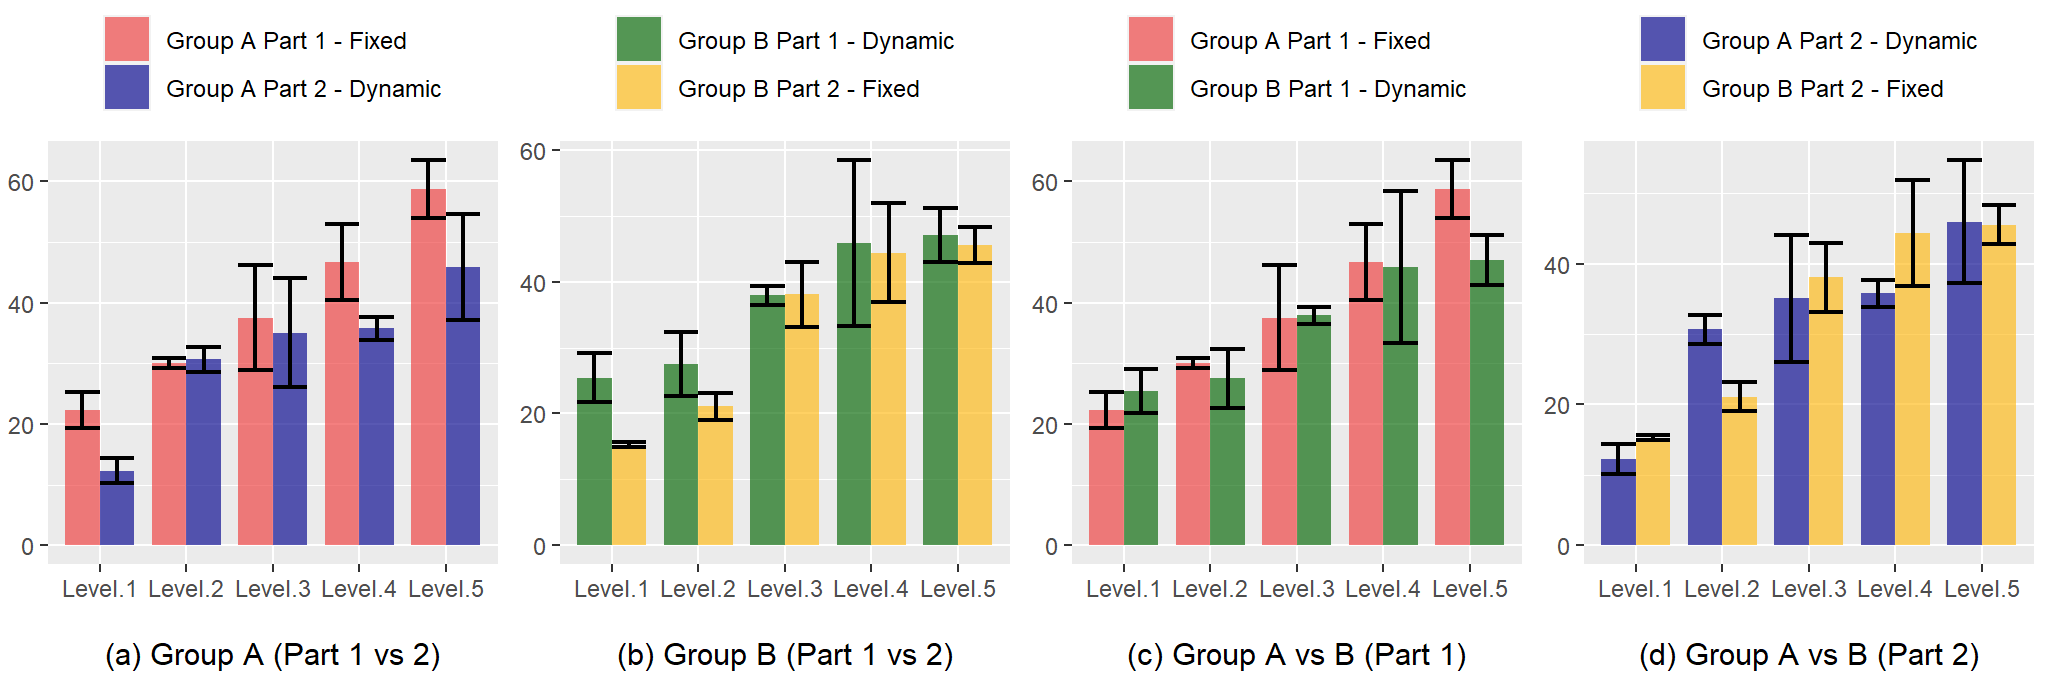
\includegraphics[width=34em]{figures/health_lost_per_encounter-veteran_players.png}
        \legend{Source: Assembled by authors.}
        \label{fig:result-metric-veterans-health-lost-per-encounter}
    \end{center}
\end{figure}

% =================================================================
% =================================================================
% =================================================================

\section{Conclusions}

% \subsection{Summary of Results}
% * Summary of Results
% * =======================

% \subsection{Limitations}
% * Limitations
% * =======================

% Calculation and adjustments based on metrics are executed between levels
% Difficulty in level 2 was always higher in DDA systems, which might show a level design issue
% Adjusments should have been tested in isolation and in groups
% Should have 5 difficulty levels for DDA, instead of 3. Because veterans and beginners should extrapolate higher and lower limits.


% \subsection{Comparison with Previous Methodologies}
% * Comparison with previous work
% * =======================

% =================================================================
% =================================================================
% =================================================================